\chapter{Domain decomposition and multi-device computation}
\label{chapter:Decomposition}

Considering the city-scale application of a model for Carlisle in the previous chapter, city-scale simulation was achievable, but the time consumed remains too long for use in a real-time simulation or forecasting capacity. To derive further performance improvements, further capabilities are required, to leverage the processing power of multiple compute devices, instead of just one. This may take the form of a traditional supercomputer architecture, with high-speed low-latency network connections between powerful discrete computers with many cores, or ideally for flood simulation, with many GPU devices available. Consistent with the approach outlined previously, it is the intention here to create a computational method which could theoretically be applied to either of these systems.

Leveraging multiple processing devices for a single simulation is no simple task, when considering the complexities of managing multiple devices of mismatched computational power, focusing on different parts of the spatial domain, and potentially within a number of discrete computer systems, connected by a network. For this reason, very few software for flood simulation can provide this functionality, and to the author's knowledge, none of those commercially available for distribution, provide this capability. Acknowledgement should be given to JBA Consulting's JFlow-GPU, built upon the work of \citet{Crossley2009}, which offers some of this functionality, but is an internal tool, not available for general resale.

There are but a handful of existing studies in which multi-GPU simulations have been attempted, for flood simulation. The work described by \citet{Saetra2012} provides a starting point and was groundbreaking, presenting a similar approach to one described later in this chapter, where timesteps are exchanged between all processing devices, delivering major performance benefits for their examples with many millions of cells. In practice, many simulations do not contain that many cells, and the requirement is as much concerning high throughput in terms of overall duration, which is a more difficult problem. Similar findings are reported in \citet{Vinas2013} and \citet{Asuncion2016}, where large domains are required to improve the weak and strong scaling effects. Previous work by \citet{Sanders2010} is also similar to the approach adopted herein, but focused on hydrological modelling using CPU-based supercomputer architectures, rather than GPUs, although the principles are comparable. The intention here is to provide software capable of accelerating as broad a range of flood scenarios as possible, thereby providing a means of operation on traditional supercomputer architectures and smaller systems, by leveraging OpenCL and other open platforms.

It is also worthwhile acknowledging the extent to which future advances in technology might negate the need for complex domain decomposition implementations. Processor clock speeds have advanced negligibly throughout the last decade, as scale and temperature becomes a constraint. However, multicore processing is increasingly prevalent, including in mobile devices, and this has largely allowed background processing and foreground to be segregated through threading, for an improved user experience. The same trend can be expected in future years until a major advance in computer processor technology is achieved. Multicore processors typically have access to a single shared memory domain, and thus decomposition is not required in the manner described herein. It is likely nonetheless that high-resolution data will become ubiquitous, and detailed physically-based catchment-scale modelling should become increasingly prevalent; domain decomposition is likely to be necessary for catchment-scale modelling for many years to come.

\section{Principles of domain decomposition in explicit time-marching schemes}

The finite-volume scheme can be considered in the form of stencil operations, for which each cell is dependent on its neighbours for a first-order solution. This is ideally suited to the architecture of GPUs, as described in earlier chapters. Achieving expedient simulation is largely dependent on a small portion of the overall code, which undertakes the calculations for the time-marching scheme; this is essentially flux calculation and updating of the cell states, followed by a reduction algorithm to identify the maximum velocity in any cell across the domain, for the purposes of satisfying the earlier-described CFL condition. This dependency on neighbouring cells presents a problem, where a straight-forward splitting of the domain would move some of those neighbours to an entirely different device and therefore memory.

The timestep then presents a further problem. The CFL condition described in Equation \ref{CFL} governs the maximum timestep through which the simulation can be advanced for each iteration. In a domain decomposition situation therefore, there are two possibilities: coordinate the timestep using the maximum velocity encountered anywhere in the domain, including across all processing devices; or manage simulations in which each device progresses at a different pace, by predicting suitable synchronisation points for data exchange. The first of these cases is the simplest, but requires data be exchanged between device after each iteration completes.

\begin{figure*}[tpb]
	\centering
	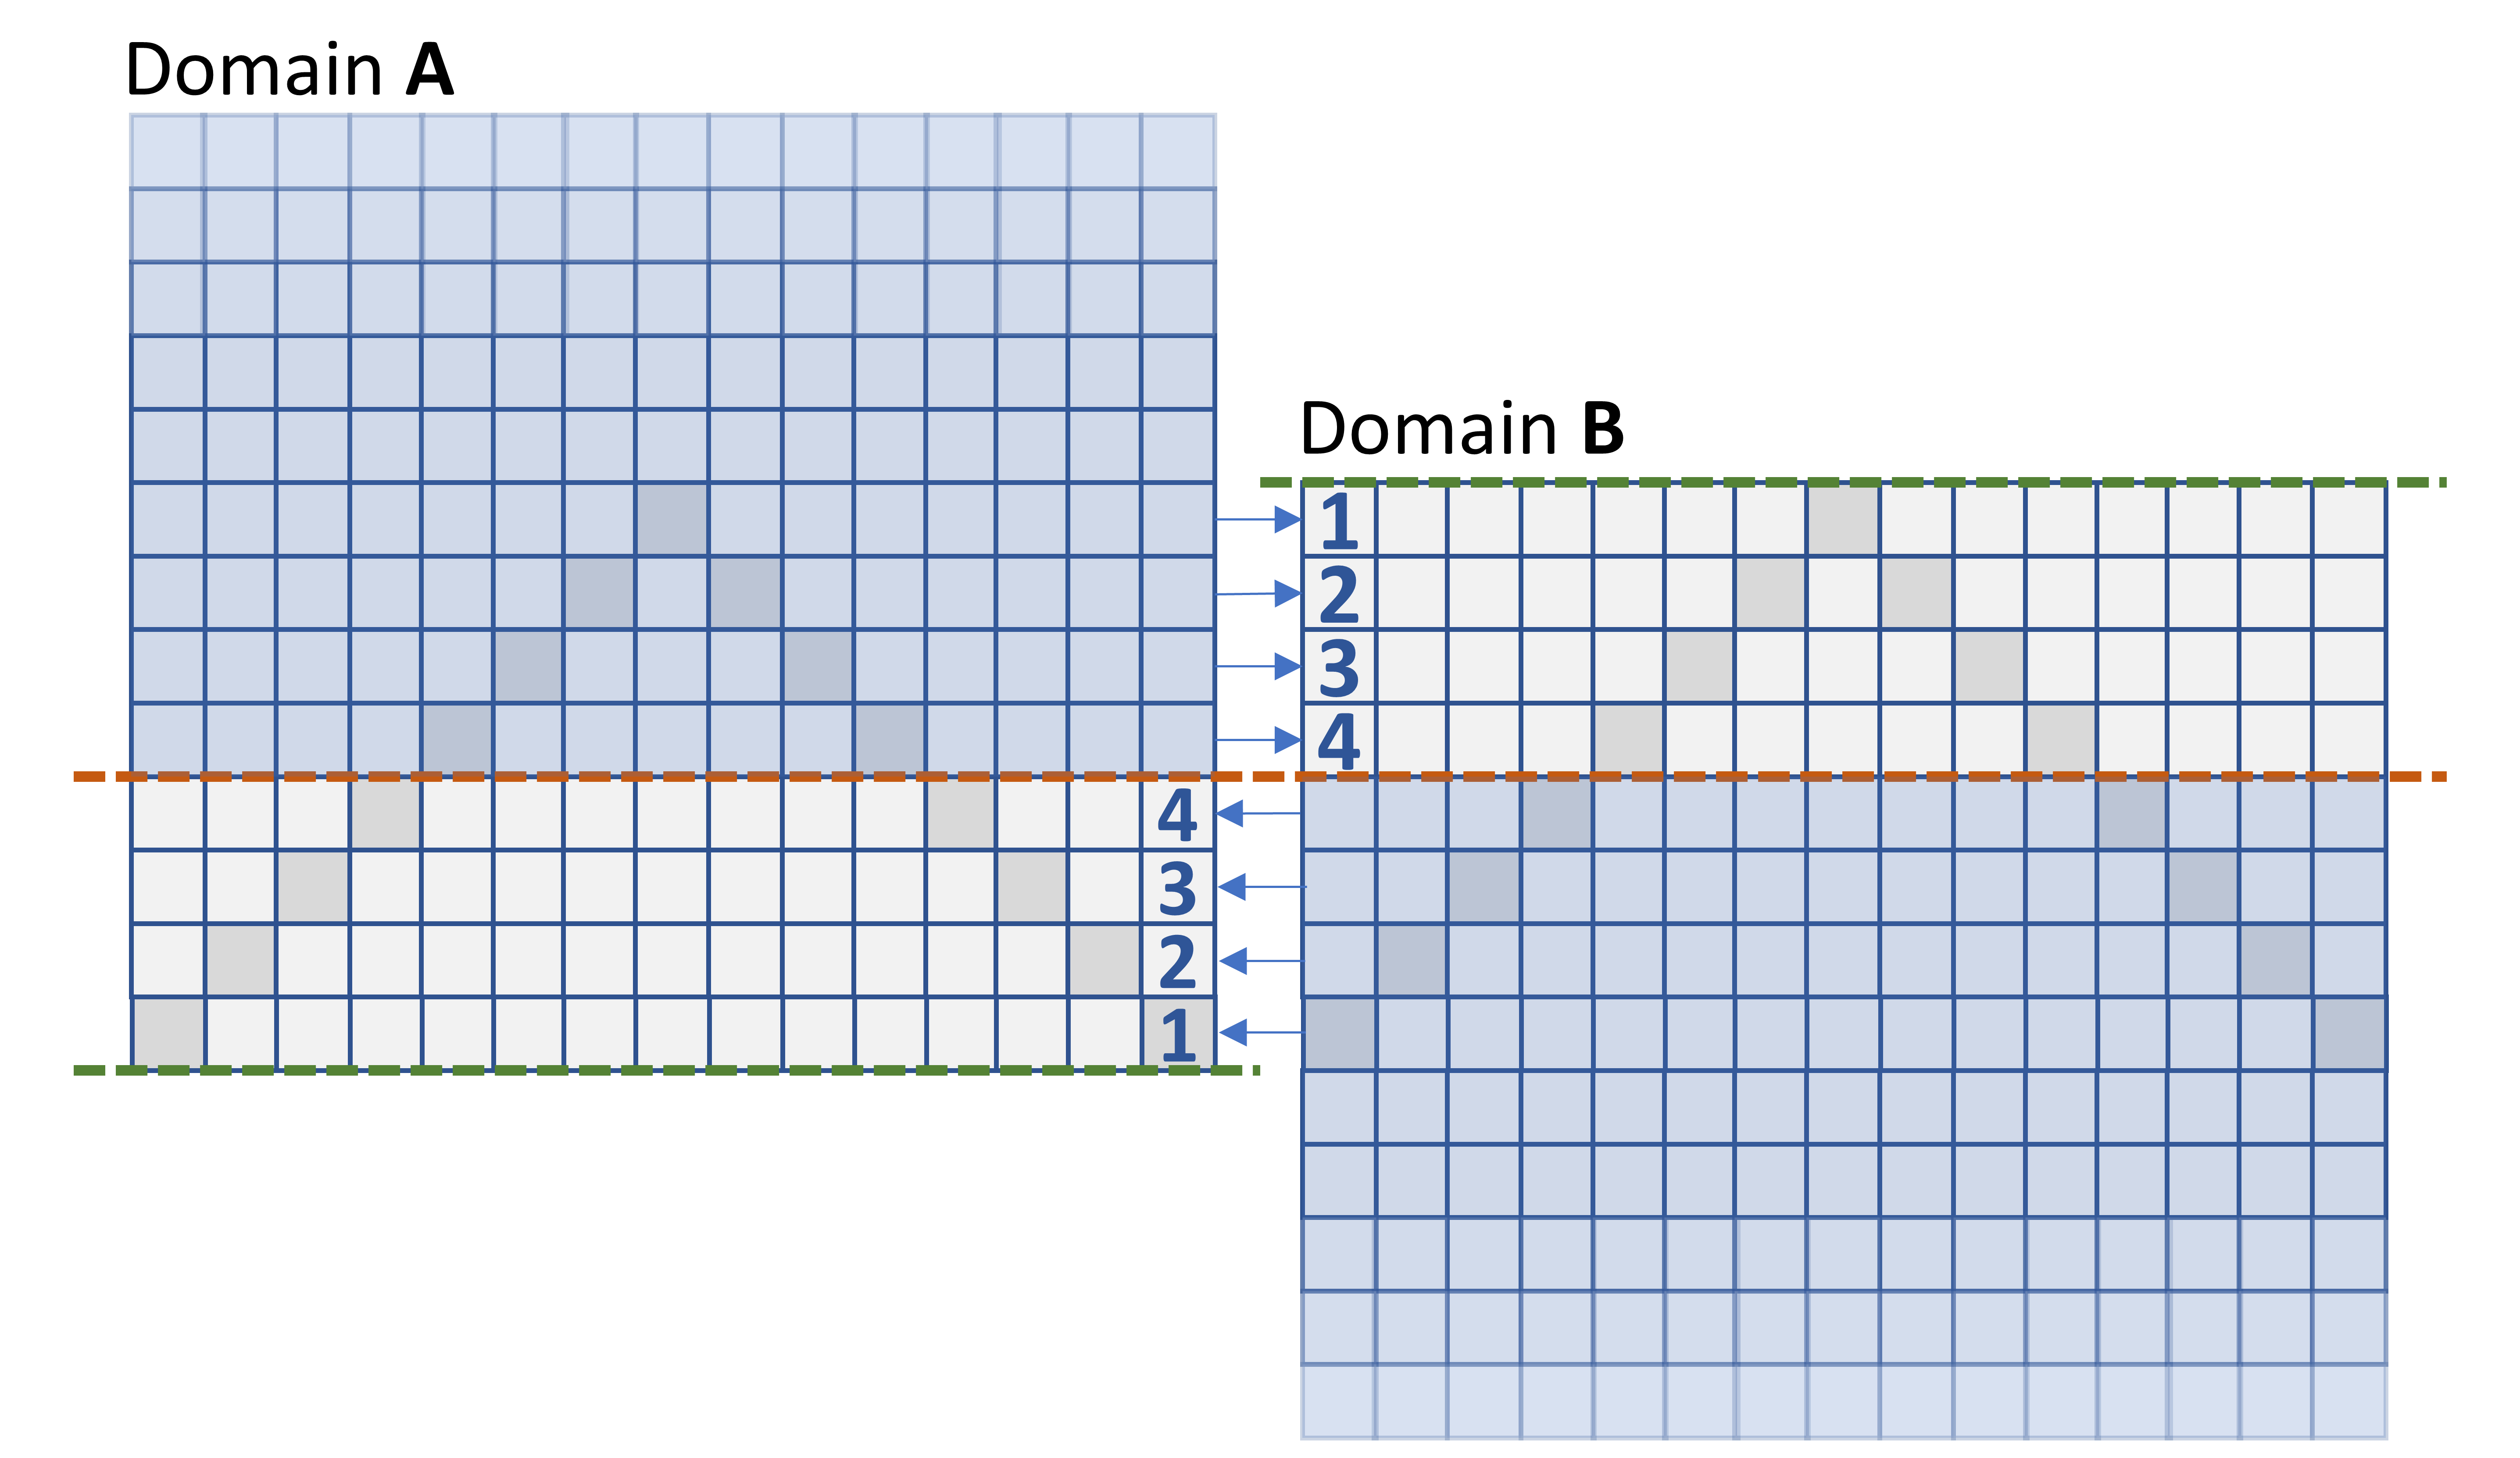
\includegraphics[width=1.0\textwidth]{decomposition-test-figures/aob.png}
	\caption{Illustration of the available overlap buffer, showing a domain split in the middle, with four rows of cells duplicated into both domains, hence each time a full synchronisation occurs these rows may be substituted with data from the corresponding region of the other domain to correct any errors from the limited knowledge of neighbouring cells.}
	\label{AOB_Description}
\end{figure*}

Taking the simplest case, where it is possible to exchange data in each iteration, the CFL condition provides the useful advantage that a discontinuity or a wave may only progress the distance of one cell during one iteration, as this is the premise of CFL, and thus reason it provides stability. Where the domains for each processing device overlap, data may be exchanged along that border such that neighbour data is always available. A minor extension to this approach, would be to overlap the domain partitions by more than a single cell, so only timestep data is exchanged at every iteration, and cell data need only be exchanged at a point prior to when the availability of neighbours would be exhausted; this number of neighbours available between the area of interest and the end of the overlap zone, will be referred to as the available overlap buffer (AOB) hereafter. This concept is illustrated in Figure \ref{AOB_Description}, where four rows of cells represent the AOB. The lack of data on cell states outside the domain under consideration causes small errors to be introduced in each iteration, but the same row is simultaneously processed as part of the other domain, because of the overlap, allowing these errors to be corrected when cell state data is exchanged. The numbers in the figure illustrate the order in which the errors propagate, one row per iteration pursuant to the CFL condition. The blue region indicates cells regarded as free of these errors, hence authoritative data source.

For the second case, in which each decomposed fragment of the domain may run independently with its own timestep, any error arising in the solution at the extremities of the domain, because neighbour data lacks currency, will only propagate by one cell at a time. This allows these errors to be corrected, providing the AOB is not spent by the time data is exchanged between compute devices. In the event overlap is exhausted, a rollback to the last saved state is required. This is nonetheless dependent on the maximum time step being calculated after each iteration, making some host bus transfers inevitable but minimizing their size. The requirement for an overlap also means a model must consist many millions of cells before decomposition to multiple devices becomes a worthwhile pursuit, because the total number of cells is increased by the procedure.

\section{A multi-device multi-nodal implementation with decomposition}

The optimisations and techniques discussed so far, have focused on using the OpenCL programming framework, and therefore can take advantage of either CPUs or GPUs with a single codebase. This portion of the code is optimized in two ways. Firstly, the code is compiled just-in time before the simulation begins, allowing model-dependent constants (e.g. the grid resolution, constraints on time steps, and some parameterisations) to be incorporated within the model code directly. Secondly, the process is implemented as a simple sequential set of OpenCL kernels representing the stencil operation, with appropriate barriers incorporated where synchronization is required across the whole computational domain.

The underlying system drivers manage the vectorization for low-level optimization, and deployment of this code on the hardware available, which need not be limited to GPUs but could also include hybrid-style processors (APUs) and IBM cell processors. Data is transferred to the device's own DRAM memory (see Figure \ref{CPUGPUArchitecture}) before computation begins, and transferred back as infrequently as possible, allowing for status updates and file-based storage of results. Transferring both instructions and large volumes of data across the host bus is far from desirable, and would represent a major bottleneck in the process if undertaken too frequently. However, as the total domain size increases, the delay introduced by latency across the host bus, as a proportion of overall computation time, becomes a diminishing portion. This presents an opportunity for domain decomposition, but only for instances where the problem size is sufficient to justify frequent data transfer.

\begin{figure*}[tpb]
	\centering
	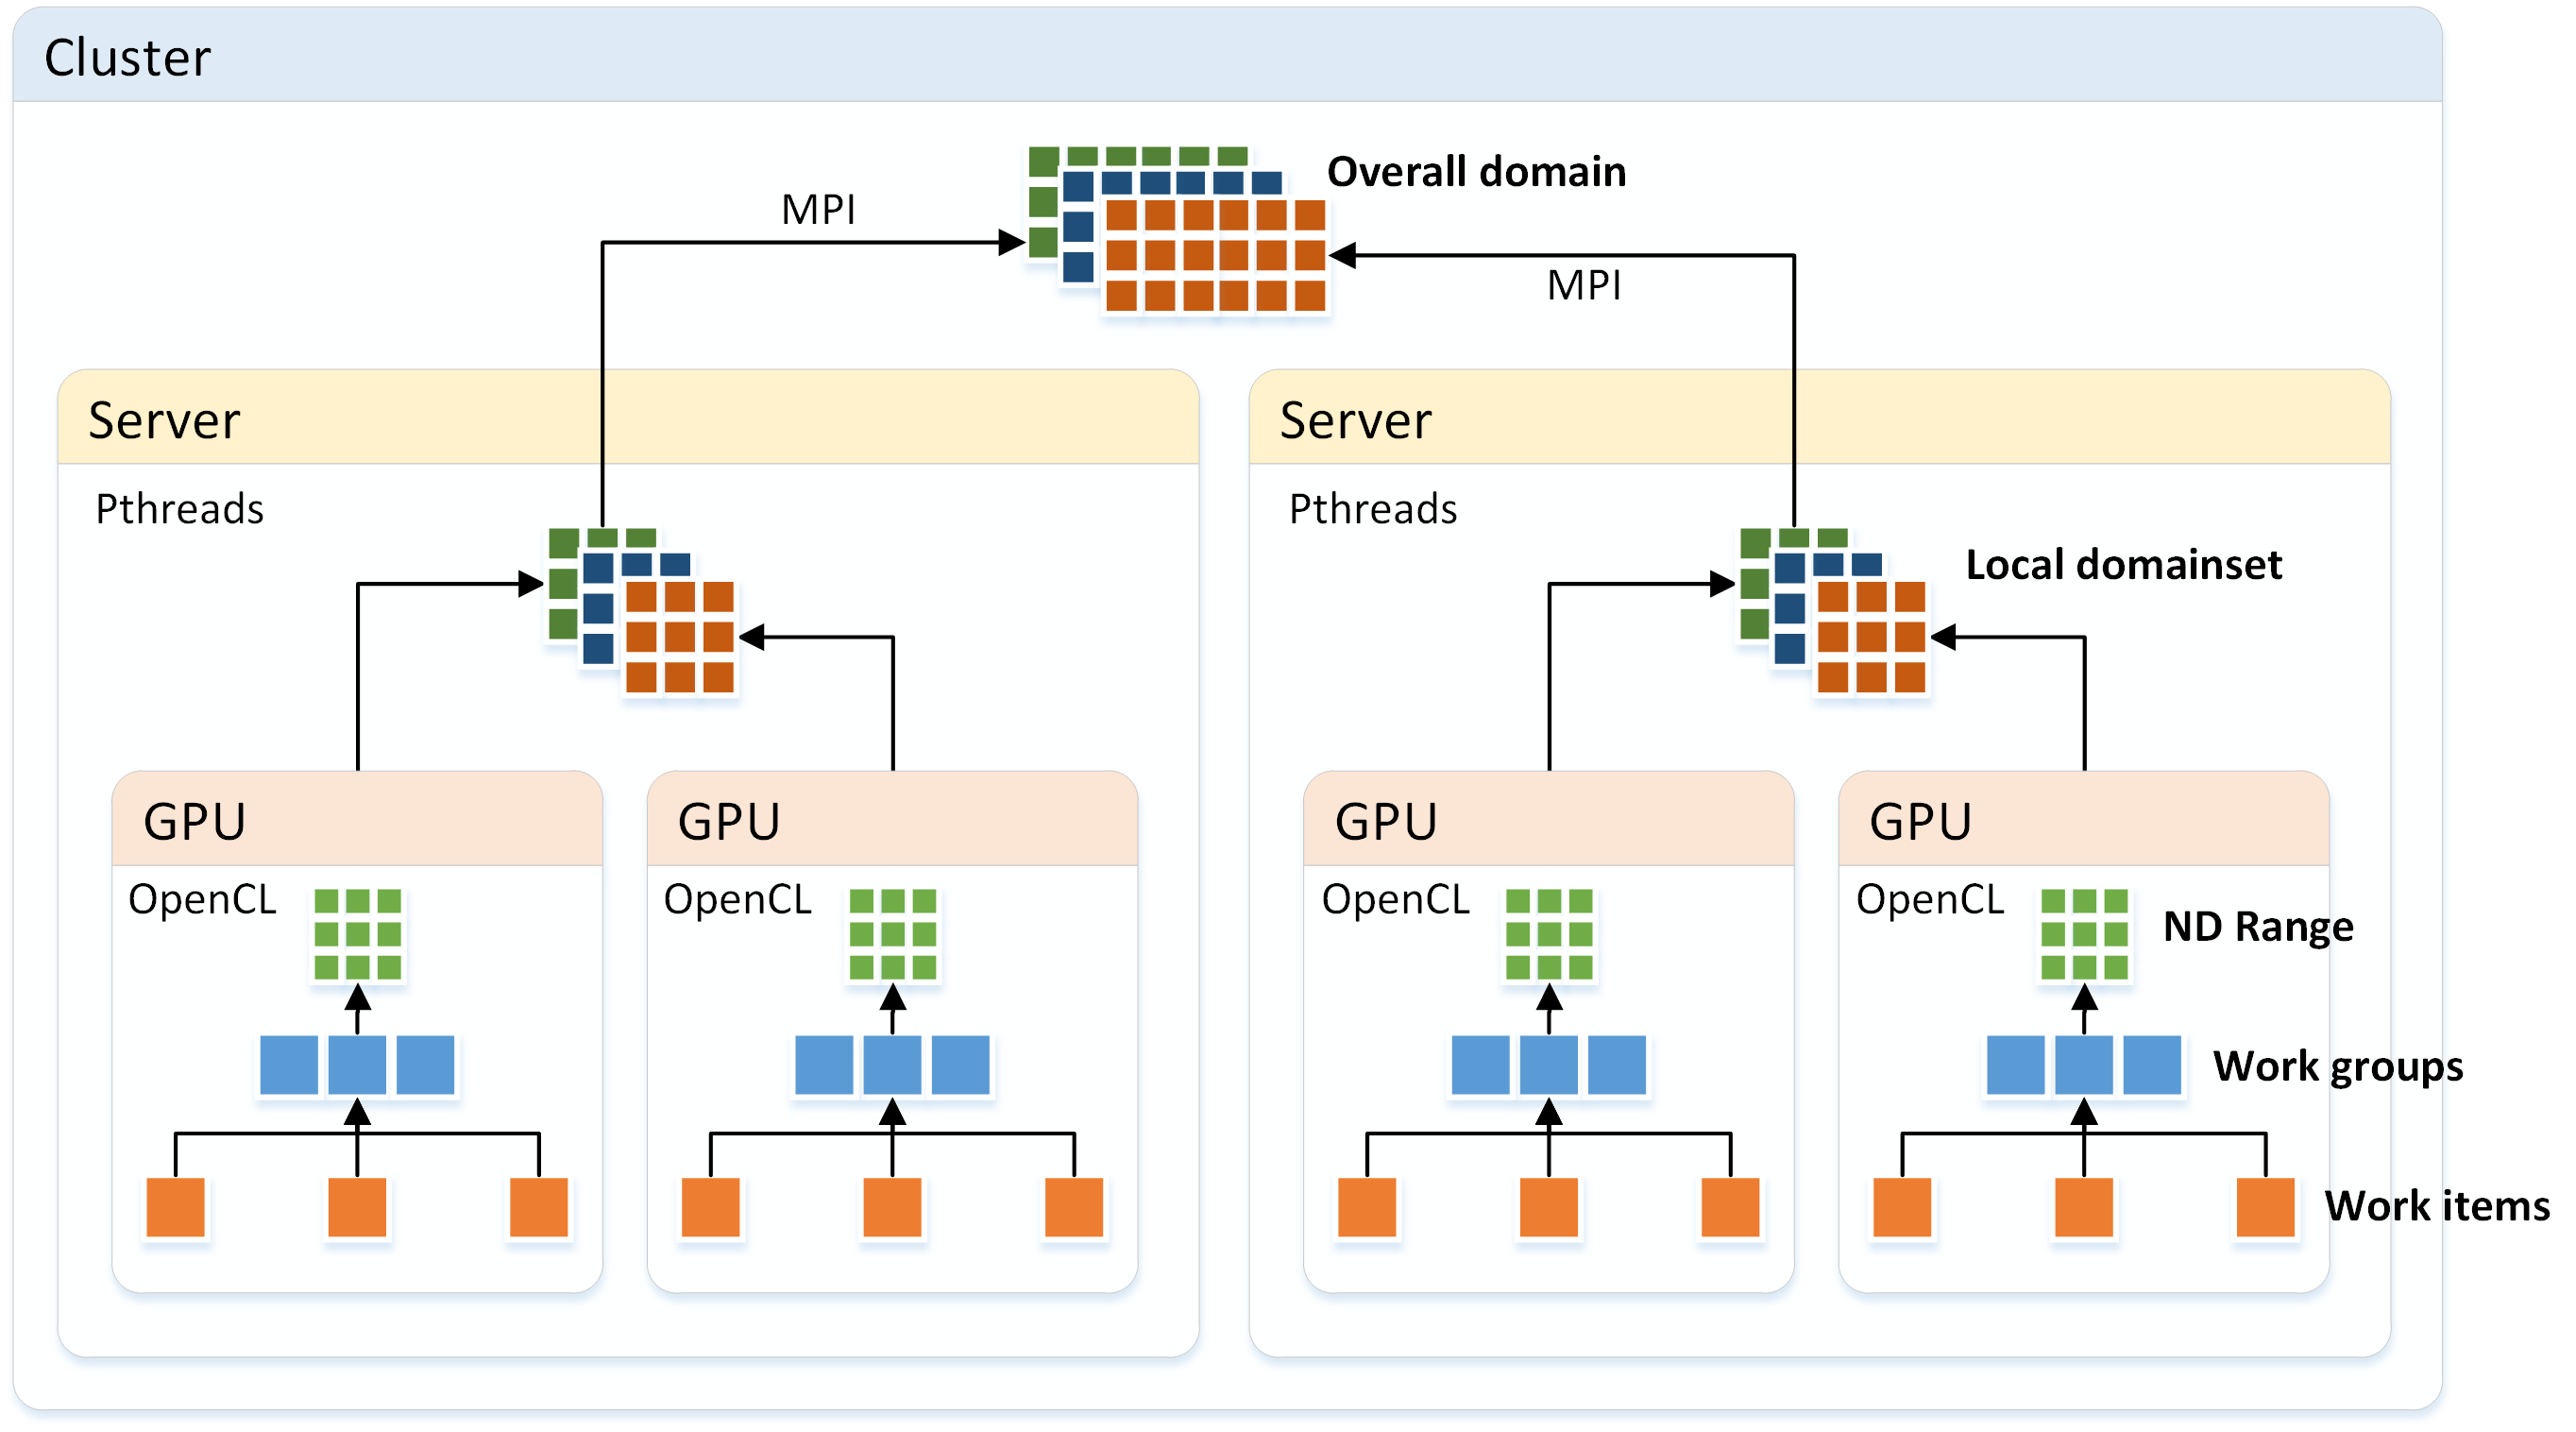
\includegraphics[width=1.0\textwidth]{mpi-figures/sync-levels.png}
	\caption{Representation of the synchronisation levels, from work groups, to device domains, servers, and the overall domain spread across several computational nodes.}
	\label{Software_Sync_Levels}
\end{figure*}

This code is further developed, to support simulations across multiple GPUs using a domain decomposition technique, and across multiple systems through an implementation of the Message Passing Interface (MPI) standard \citep{MPI2009}. A separate CPU thread is used to manage each compute device, accepting some idle resource for a short period of time, for example in a tidal inundation model an entire sub-domain could be dry before the wave arrives. The general form for the multiple levels of data synchronisation is shown in Figure \ref{Software_Sync_Levels}, where data is exchanged between discrete computer systems using MPI, and within a single computer system, a separate CPU thread is used to coordinate for each device, with each allocated its own memory space.

The message passing interface (MPI) is a software standard for communication between processes operating either on the same machine, or connected via a network. It is commonly applied in supercomputing, where Infiniband, a communication standard capable of achieving throughput $\gtrapprox120$ GBit/s and latency $\lessapprox0.5$ microseconds, or comparable network speeds allow these messages to be passed with great speed and minimal latency, and the algorithms associated with some operations can in some cases be processed and assisted by network hardware, such as a reduction to find the largest or smallest value from those held by each node. There are a number of implementations of the MPI standard, many of which are open-source; herein, MPICH (\url{https://www.mpich.org/}) is adopted. There are numerous similarities between the functionality afforded by MPI, and that which exists in the OpenCL 1.2 standard, such as the commands to send and receive from memory buffers, and initiate barriers where all concurrent programs must wait for all others to reach the same point, for synchronisation. In the case of MPI over networks or between processes, even though extremely high speeds may be available, for applications which exchange large volumes of data on a regular basis, there is likely a limit beyond which no further performance gain can be achieved, in part because of the overheads of dealing with each of these operations, as a proportion of the productive processing time.

Owing to the speed constraints of the PCI bus, the means of transferring data from the main system memory to peripheral devices such as GPUs, these exchanges are computationally expensive, and so to reduce the frequency required, it is not necessary to exchange data after every time step, provided there is a sizeable overlap between the two sub-domains. 

\section{A temporally-decoupled implementation for decomposition}

The unproductive period while a processing device is consuming less than its full capacity while waiting for other elements to complete, is known as blocking, and is largely unavoidable. The issue comes when scaling simulations to use hundreds of processing devices, where not only is blocking required on a regular basis, it becomes a major complexity for the whole system, albeit one which can largely be handled by the algorithms and routines provided by MPI. The greatest source of blocking in the implementation described thus far in this chapter, is the exchange and identification of an appropriate timestep, to guarantee numerical stability. It follows then, that if timesteps need not be synchronised globally across the whole system, there is an opportunity to reduce blocking operations. 

The reality is slightly more complicated however: decoupling the timesteps between fragments of the whole domain, could lead to large disparities between the timesteps used, which are primarily a function of the depth and velocity in the fragment. A tidal inundation simulation for example, could have swathes of the domain initially completely dry, therefore requiring a single iteration to advance the simulation by the same amount as a hundred iterations for the fragment containing the sea, constrained by the CFL condition. The method that follows therefore, does not seek to remove the blocking, but merely reduces the amount of unproductive processing. Hypothetically, with some clever management of the simulation, by removing these unproductive iterations from the process other operations could take place instead. More than one fragment of the total domain could be assigned to a single processing device, such as large areas with minimal inundation, which would benefit from the scheme exiting early when dry cells are detected; this is a step further than the implementation described herein goes, but may be an opportunity for the future.

\begin{figure*}[tpb]
	\centering
	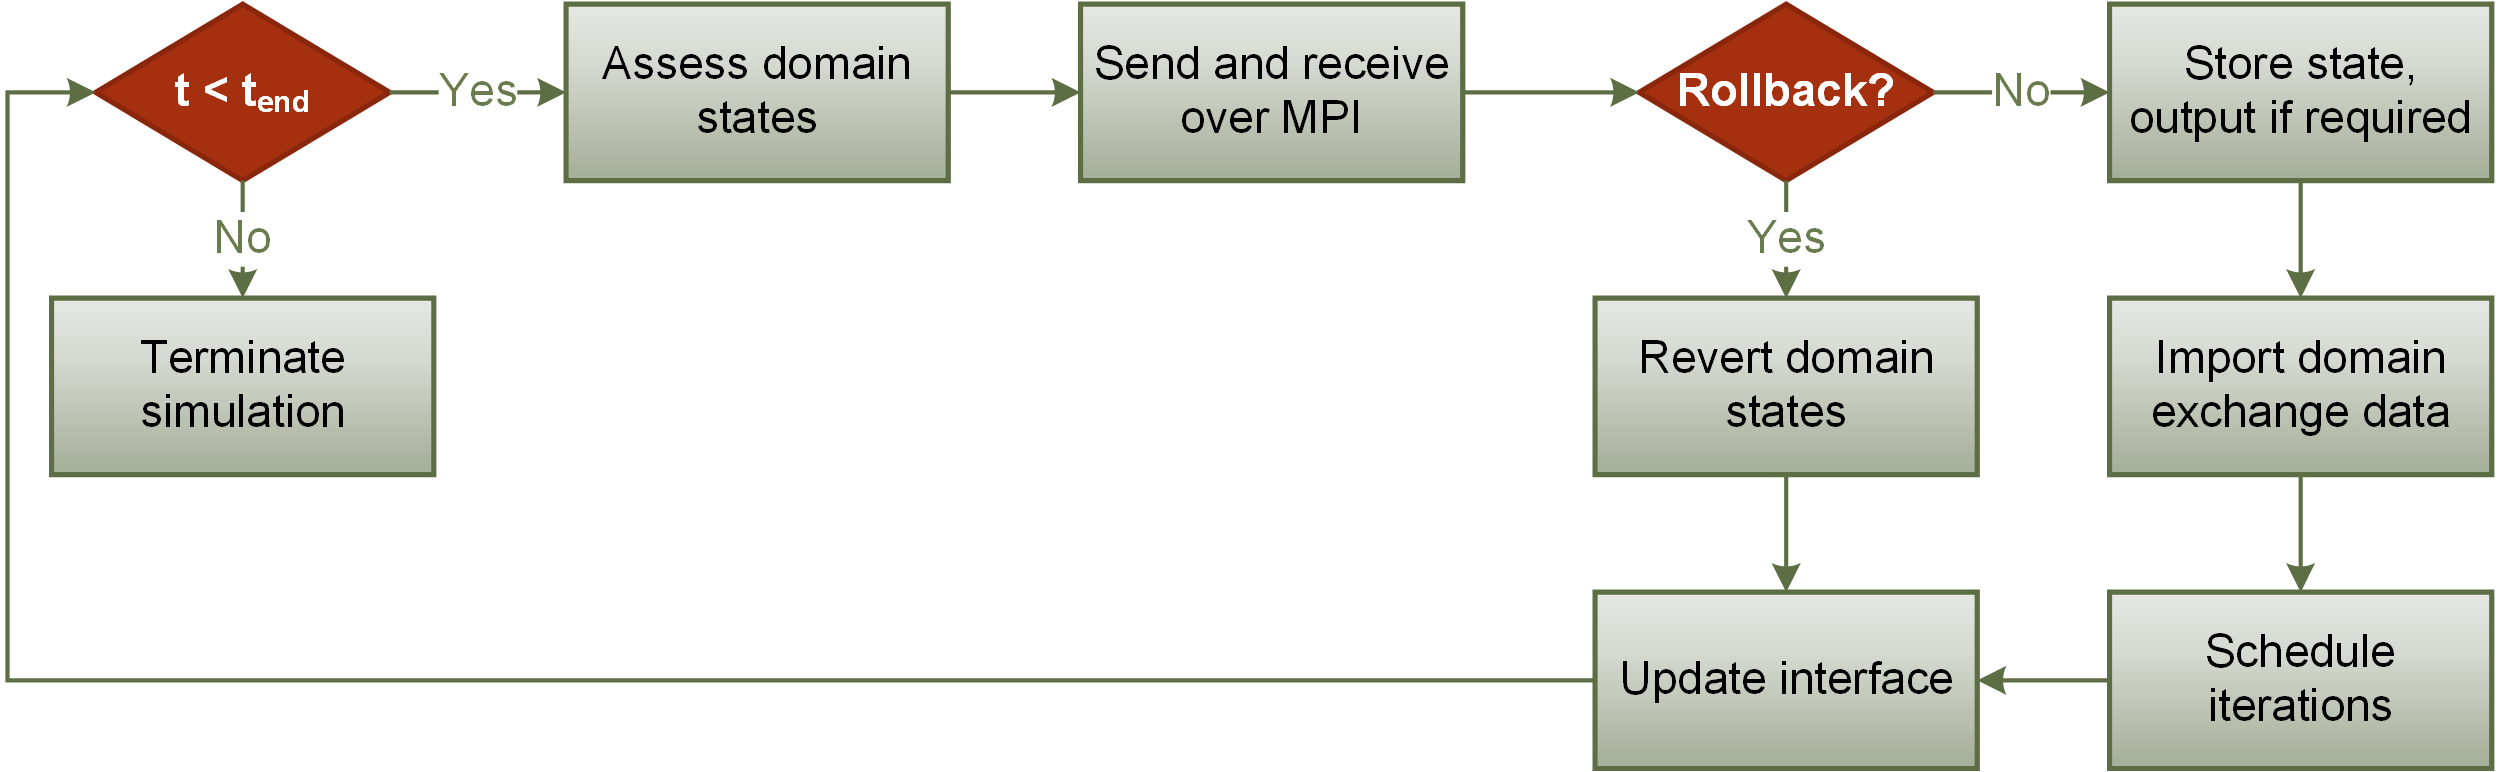
\includegraphics[width=1.0\textwidth]{mpi-figures/mpi-flowchart.png}
	\caption{Simplified representation of the processes involved in a temporally decoupled implementation, in which domain states may need to be reverted if synchronisation is not possible.}
	\label{Software_MPI_Flow}
\end{figure*}

In order to decouple the timesteps, an appropriate point in the future needs to be identified, at which the data may be exchanged. At this point, all domain fragments must be at the same point in time for the simulation. Calculation of an appropriate synchronisation point in the future is no simple task, and must be an estimate.

The approach adopted for determining an appropriate synchronisation point is:

\begin{itemize}
\item if the overall simulation time has progressed by $< 10^{-5}$ seconds, or the last known batch did not deliver any successful iterations, then revert to running a single iteration as synchronisation or an error may be imminent; otherwise
\item subject to the caveat, that the proposed synchronisation point should not be less than one timestep (per the CFL constraint calculated during the previous run) in the future, unless this would exceed a required point (i.e. when output files should be written to disk, or the simulation should terminate); then the synchronisation point is the current simulation time, plus the average timestep for each iteration since the last synchronisation, multiplied by the number of cells in the buffer, and the user-configured percentage of the buffer to consume.
\end{itemize}
This should provide a point likely to leave some of the buffer free (per the configuration), but this is not guaranteed, as the previous batch may not be representative of future flow conditions.

The performance achievable is highly sensitive to the user-configured spare AOB, where setting this value too low will result in an excessive number of rollbacks for the entire domain state, every time shocks and major variations in flow conditions are encountered, but too high will fail to fully utilise the processing power available, with potentially redundant cycles depending on the method employed for queueing iterations on the processor. There is also a coordination overhead associated with these calculations, and pausing elements of the simulation while a proposal is calculated at each node, and the lowest of these identified from all of the domains in a simulation. The above method is considered na\"ive, and could likely be improved with further tuning options, or a degree of adaptivity to deal with varying flow conditions, such as in a defence failure, where volatility in wave speeds is concentrated immediately following the failure.

If the AOB is exceeded, a rollback is required. Following each successful batch, the cell state data is transferred in its entirety from the processing device to the host device, which is oftentimes unused (apart from when output files are required) but necessary in case of rollback. A rollback entails copying the host-side cell state data back to the processing device, overwriting the current simulation time, and scheduling a timestep calculation using these previous cell states, before further fluxes are calculated. The rollback is required on all processing devices, hence the procedure is treated as a blocking operation, where no device will schedule further flux calculation until all devices have reported they are ready. Consequently, rollbacks are extremely expensive operations, especially when the coordination is across network devices.

A final consideration with temporal decoupling, especially in progressive flood events or tidal scenarios, is one subdomain may require considerably more iterations than another. Each iteration contributes a degree of numerical dispersion, resulting from both the numerical scheme employed, and the rounding of floating-point values under the IEEE-754 standard methods \citep{InternationalOrganizationforStandardization2011}. This is often not a cause for concern, but in some simulations, such as the sloshing parabolic bowl considered in Chapter \ref{chapter:NumericalValidation}, the cumulative effects can be significant. The different magnitude of numerical dispersion could potentially induce shocks at the seam of each subdomain, hence judicious and conservative application is required when employing this method.

\section{Software structure}

Considering all aspects of the domain decomposition, numerical scheme, and heterogeneous processing, the implementation of this software in a manner sustainable for further development becomes of paramount importance. The software is implemented as object-oriented code, which is illustrated in Figure \ref{Software_Class_Final}. Full implementation details and additional information may be found within the code and associated comments  (\url{https://github.com/lukessmith/hipims-ocl}). In general terms, the software is structured:

\begin{figure*}[p]
	\centering
	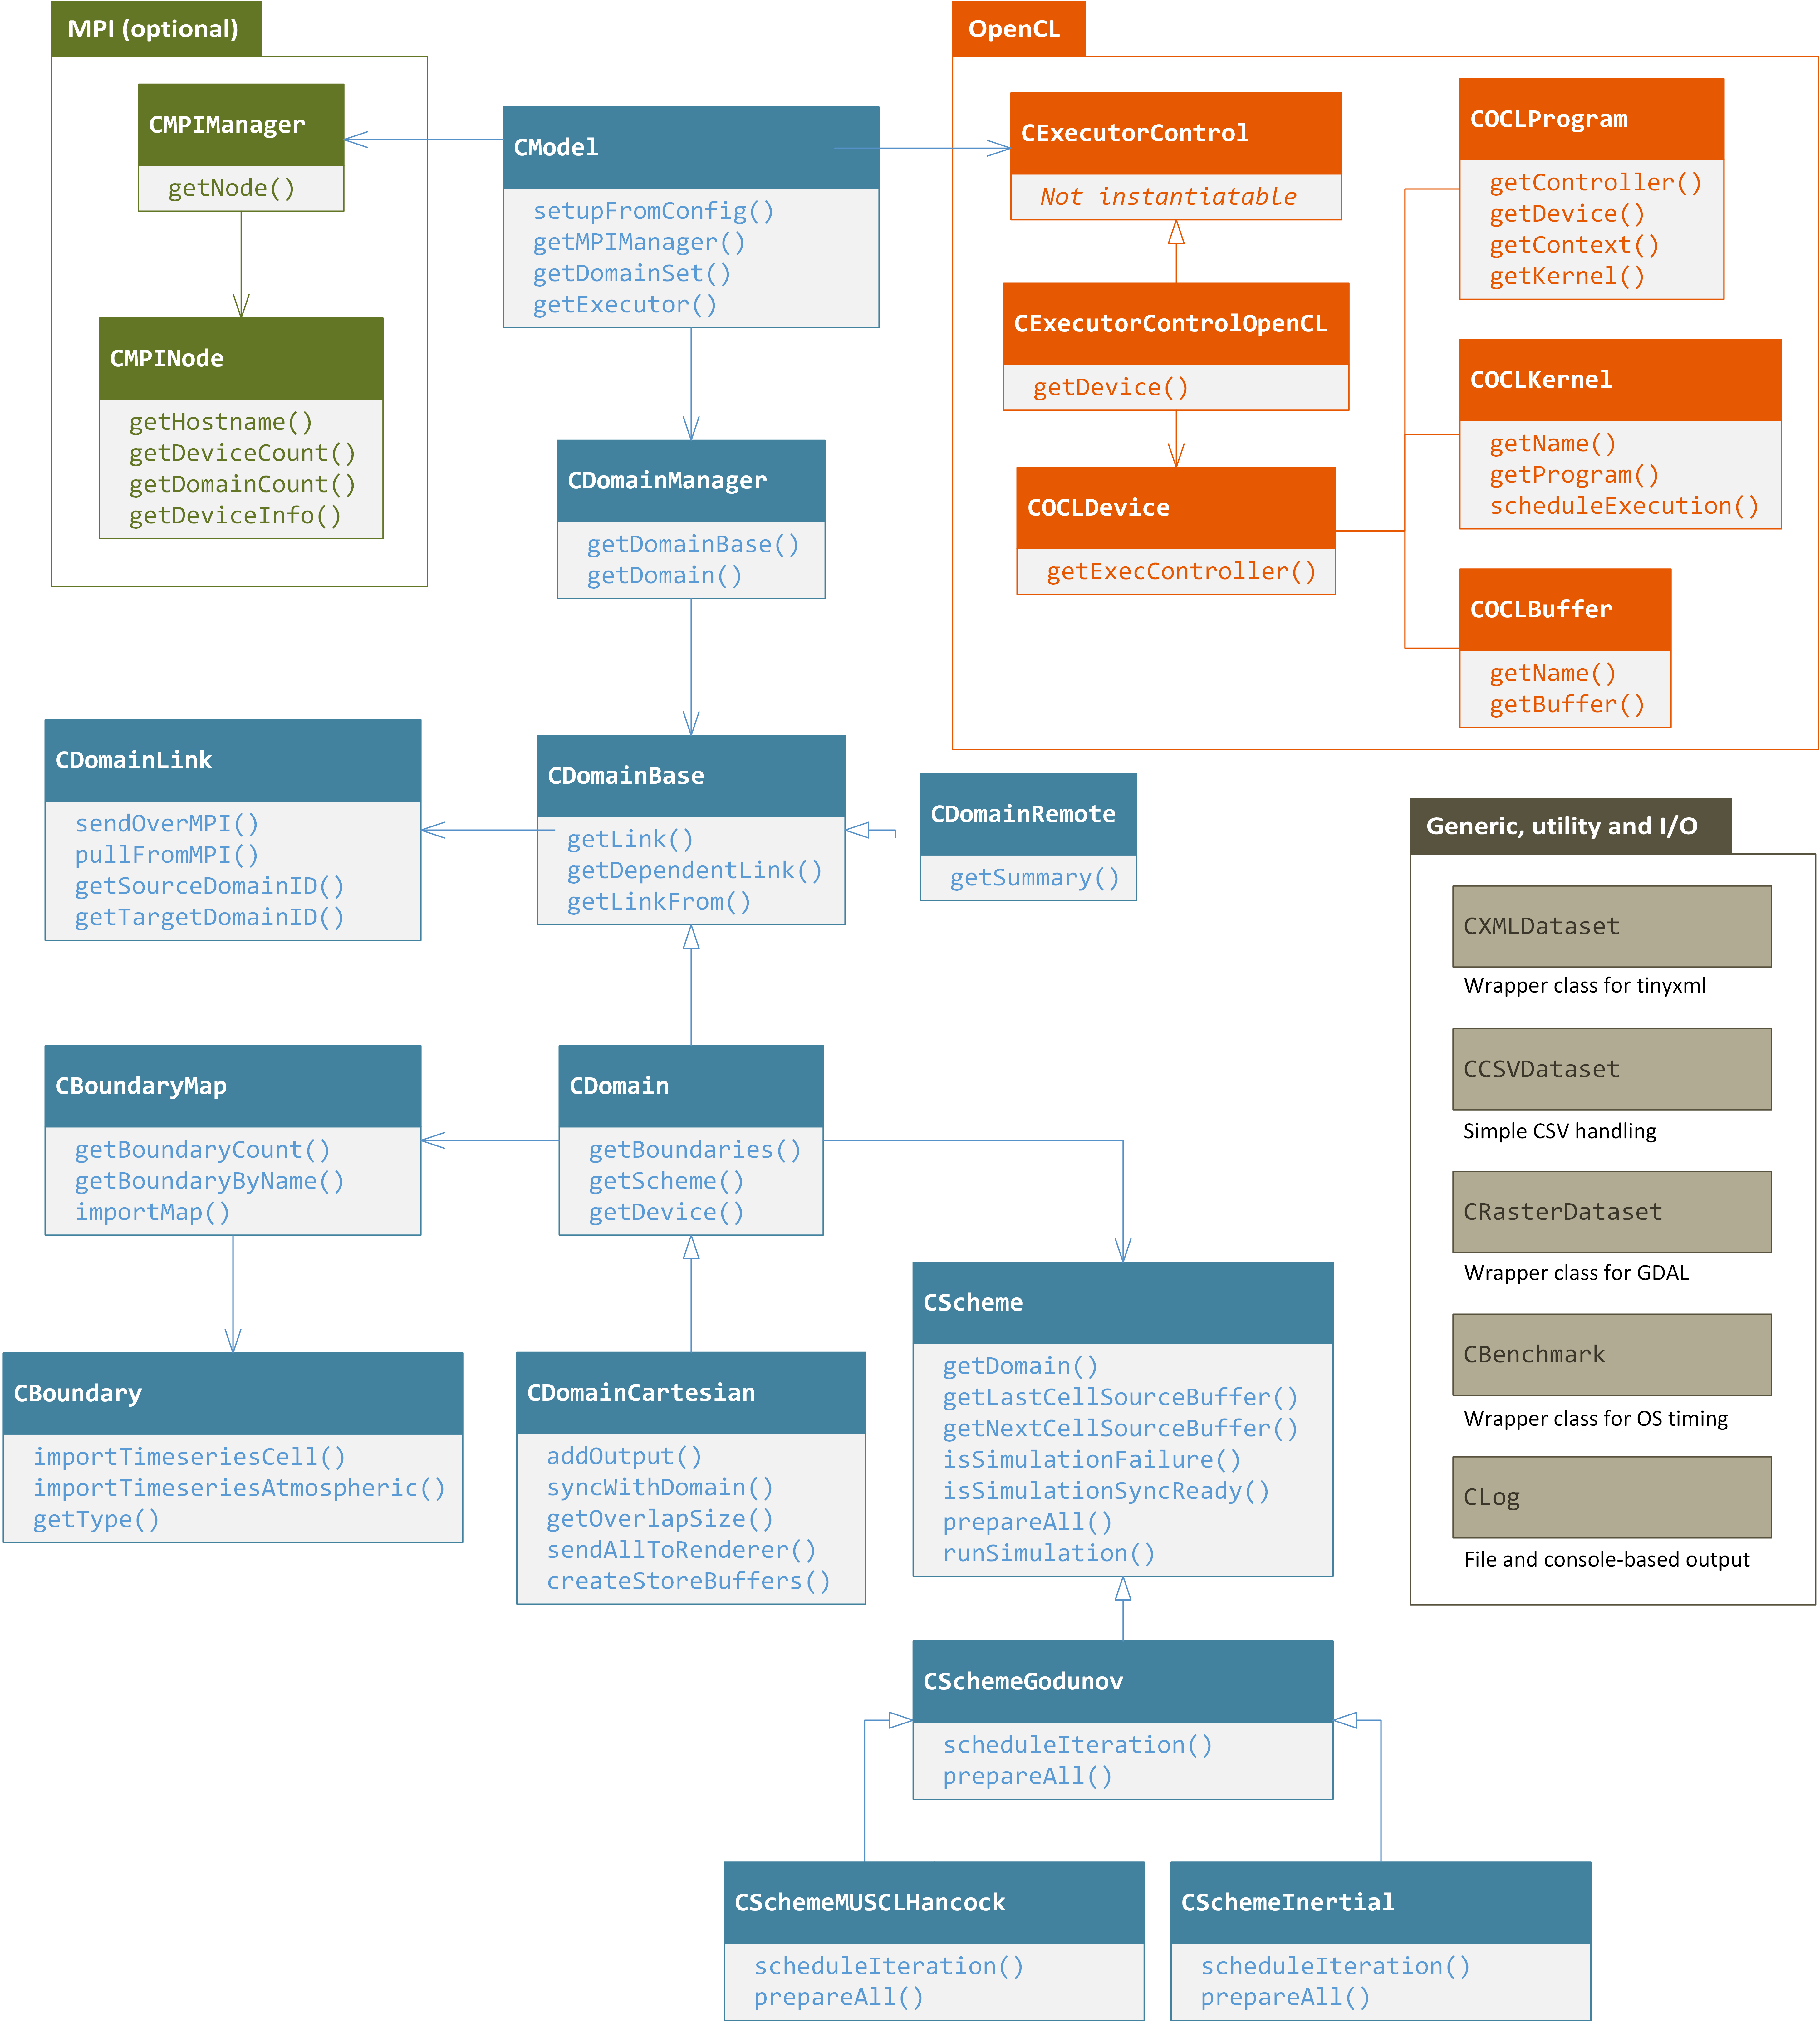
\includegraphics[width=1.0\textwidth]{mpi-figures/class-diagram.png}
	\caption{Simplified representation of the software structure, showing classes and some of their relationships.}
	\label{Software_Class_Final}
\end{figure*}

\begin{itemize}
	\item A model class (\texttt{CModel}) which provides access to all domain data and configuration for a simulation, which may be associated with an executor (i.e. the OpenCL executor for the work herein) for mapping to processing devices, and the MPI manager for internodal communication.
	\item An MPI manager (\texttt{CMPIManager}), which holds information concerning all of the nodes involved in the simulation, such as its devices and hostname, for logging and coordination purposes, within \texttt{CMPINode} instances.
	\item An executor controller (\texttt{CExecutorControl}) which is only used for OpenCL herein, but could potentially be expanded for other high-performance computing frameworks (e.g. CUDA) with some work, although much of the underlying numerical scheme code is OpenCL-specific. The \texttt{CExecutorControlOpenCL} instance provides access to the processing devices on the machine, as \texttt{COCLDevice} instances. For any specific simulation, a bespoke program is created (with model-specific constants compiled in) and managed through \texttt{COCLProgram}, with the code elements accessed and scheduled by \texttt{COCLKernel}, and memory on the processing device marshalled by \texttt{COCLDevice}. These latter classes also interpret OpenCL errors raised, and help ensure resources are cleaned up when no longer required.
	\item A number of utility classes called upon elsewhere in the program (per the programming paradigm of composition over inheritance), used for reading the XML file format (\texttt{CXMLDataset}), comma-delimited files (\texttt{CCSVDataset}) used for timeseries data, raster datasets (\texttt{CRasterDataset}) which are then handled by the GDAL library, logging to the console and files (\texttt{CLog}) and OS-independent timing of operations (\texttt{CBenchmark}).
	\item A base class for all domains, which is used also for MPI simulations, where a domain may actually exist and be controlled by another node within the network, but all nodes require an awareness of domains across the network to be able to synchronise data. Domains which exist locally are addressed by \texttt{CDomain}, and the only Cartesian domain type, currently the sole implementation (\texttt{CDomainCartesian}). Where domain decomposition exists, links are automatically created, and managed using \texttt{CDomainLink}, which extracts data from the domain where the overlap exists, and broadcasts this information across MPI to the relevant target nodes.
	\item All local domains have a \texttt{CBoundaryMap} which manages all types of boundary condition (uniform, spatiotemporally varying, and cell-specific). Each type of boundary has its own management class, responsible for loading the timeseries and spatial data, and provisioning memory on the processing device for this to reside in. This detail is omitted from Figure \ref{Software_Class_Final}.
	\item A scheme implementation, which may be first- or second-order, is managed by the \texttt{CSchemeGodunov} and \texttt{CSchemeMUSCLHancock} class (which inherits the first-order elements as a base, then supplements the additional computational steps). The scheme class is responsible for managing the time-marching, determining when data should be exchanged and written to disk, and the scheduling of work to the relevant processing devices.
\end{itemize}

A final consideration within the software design, is to ensure each device is managed by its own thread, allowing concurrent execution of the management processes, and thereby avoiding any slowdown of the heterogeneous element of the simulation.

\section{Validation and testing of the domain decomposition algorithms}

\begin{figure*}[tbp]
	\centering
	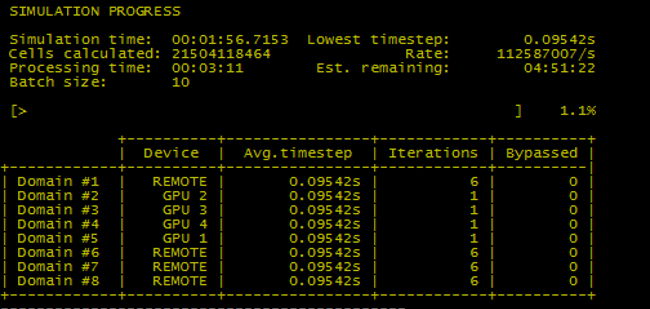
\includegraphics[width=0.92\textwidth]{decomposition-test-figures/screenshot-remote.png}
	\caption{Screenshot of the console output during a simulation using MPI between two servers with four GPU devices each.}
	\label{TestResult_Screenshot_8Domain}
\end{figure*}

The software's ability to decompose domains and synchronise data correctly between them, at the appropriate time, has been tested repeatedly during use. However, for the purposes of software testing, a limited number of identical processing devices were available, hence performance figures reported herein will use a maximum of three processing devices, all of which have identical specifications. Simulations involving up to eight processing devices were tested successfully, as shown in Figure \ref{TestResult_Screenshot_8Domain}, where two servers with four GPU devices each are used for a single simulation.

\subsection{Lake at rest}

The same test and parameterisations as found in Chapter \ref{chapter:NumericalValidation} are used here, however with a variety of grid resolutions. Whilst this test should not produce any movement of the water levels, it nonetheless requires flux calculations in all cells except the island in the centre (which is dry). It is therefore a useful performance test.

\begin{figure*}[p]
	\centering
	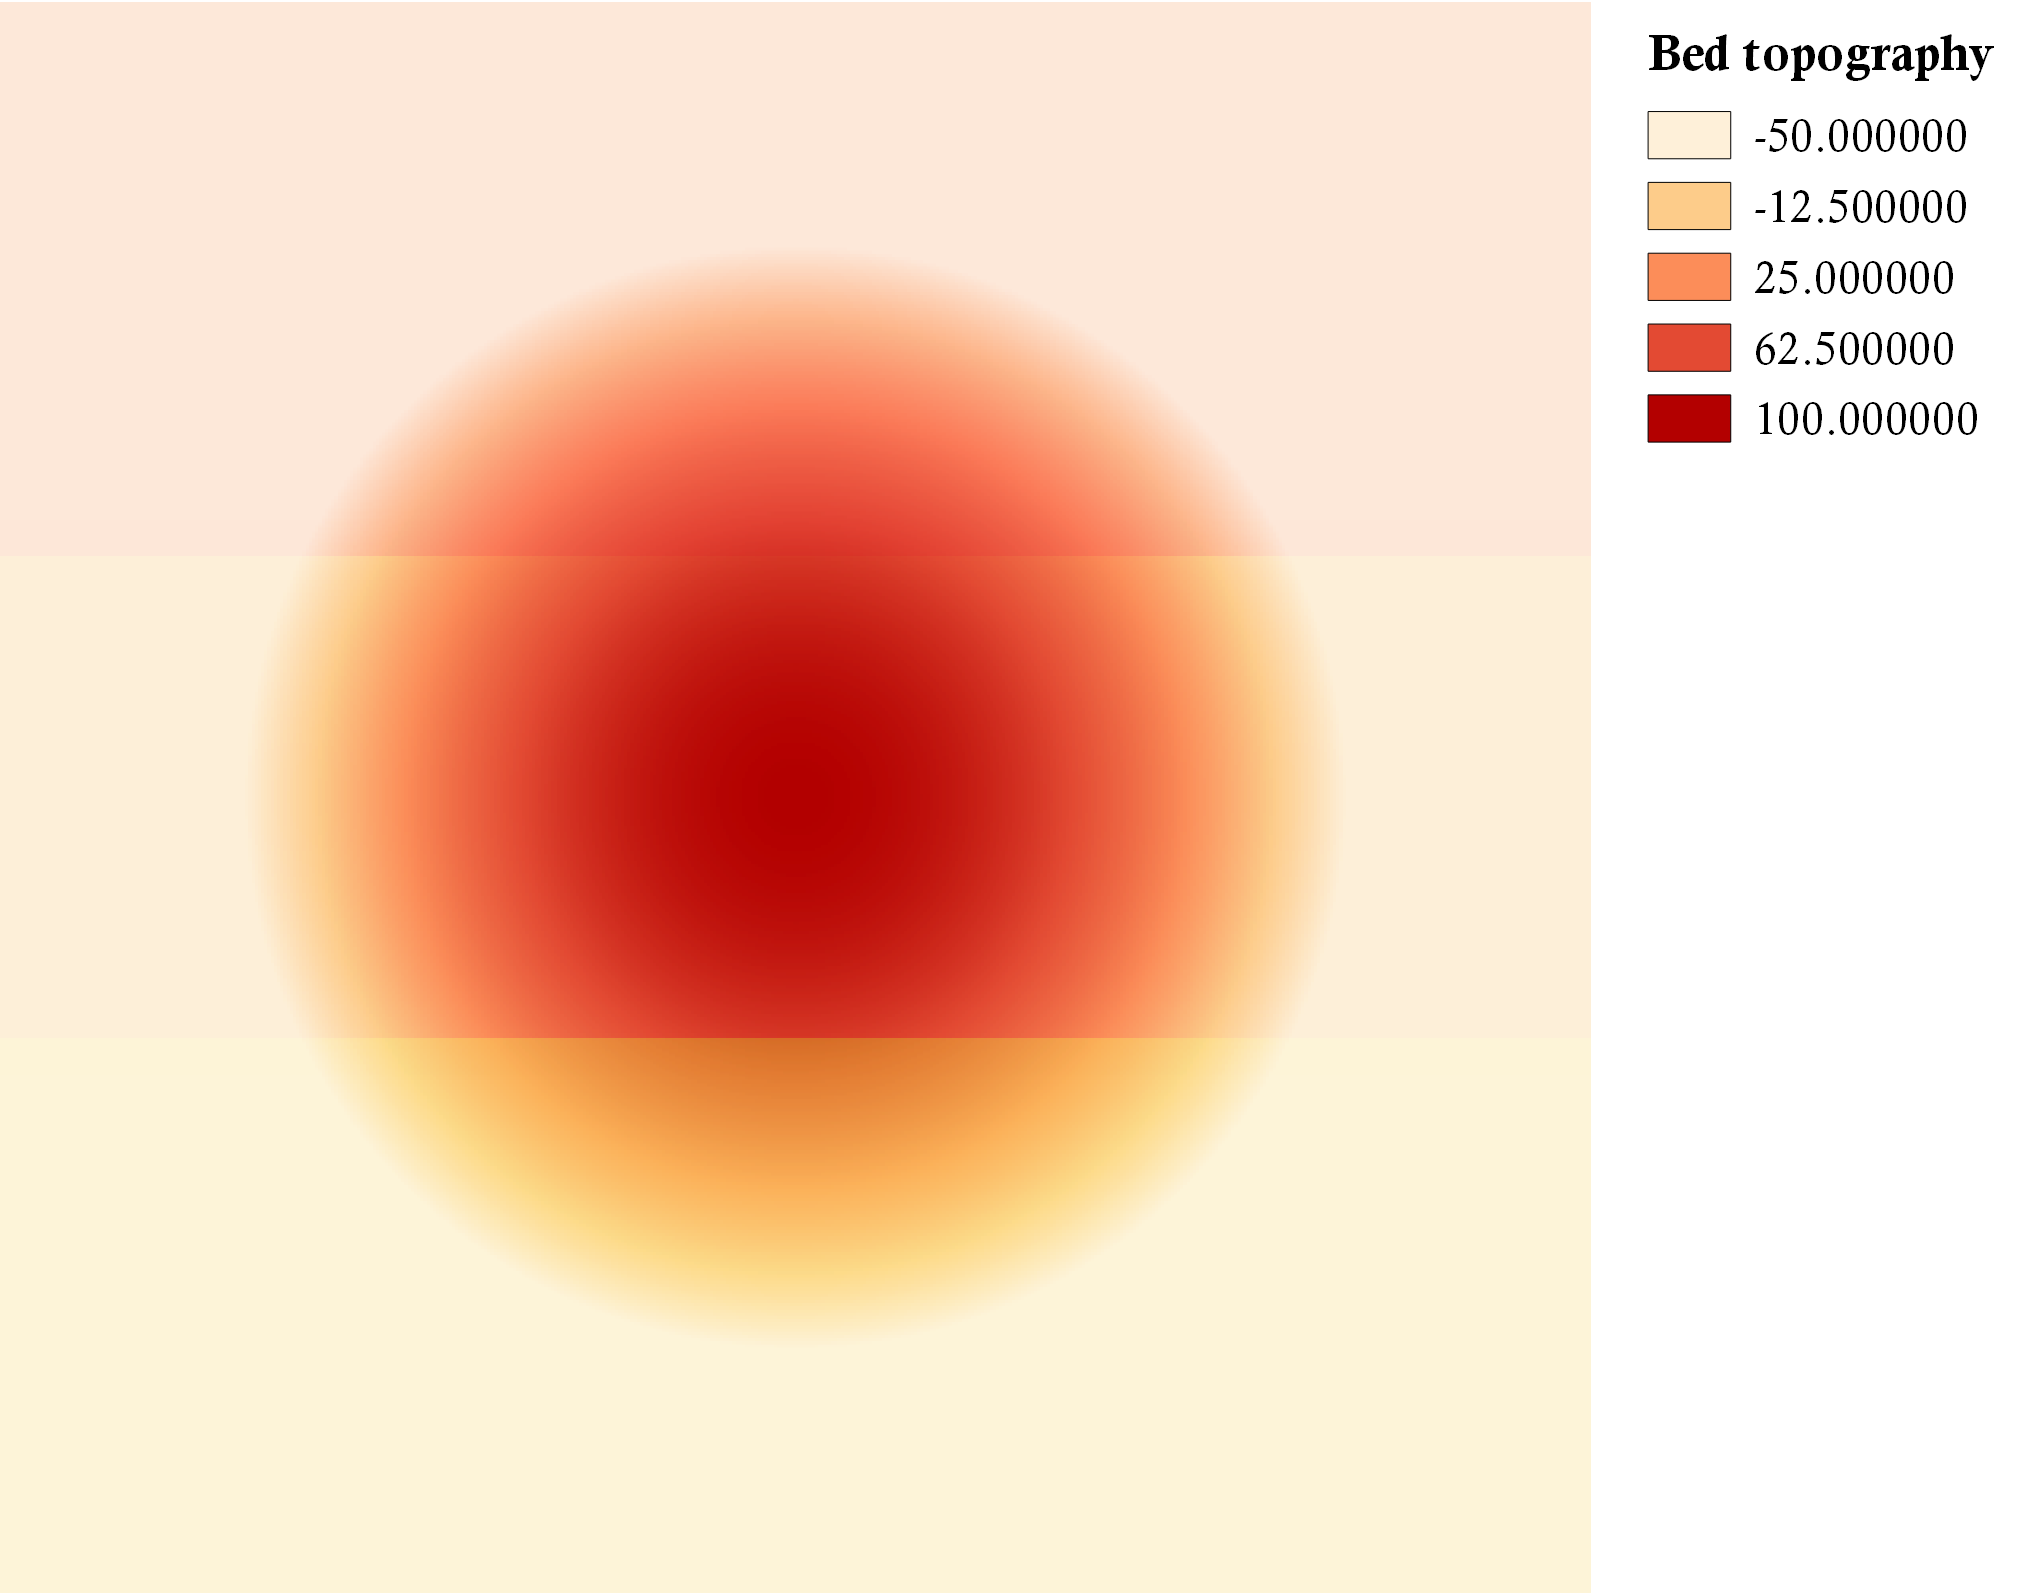
\includegraphics[width=0.85\textwidth]{decomposition-test-figures/static-lake-topography.png}
	\caption{Bed topography used for the static lake test with three devices, in which a tint has been applied to each of the subdomains to show the zones of overlap.}
	\label{TestResult_WellBalanced_Decomposed_Domains}
\end{figure*}
\begin{figure*}[p]
	\centering
	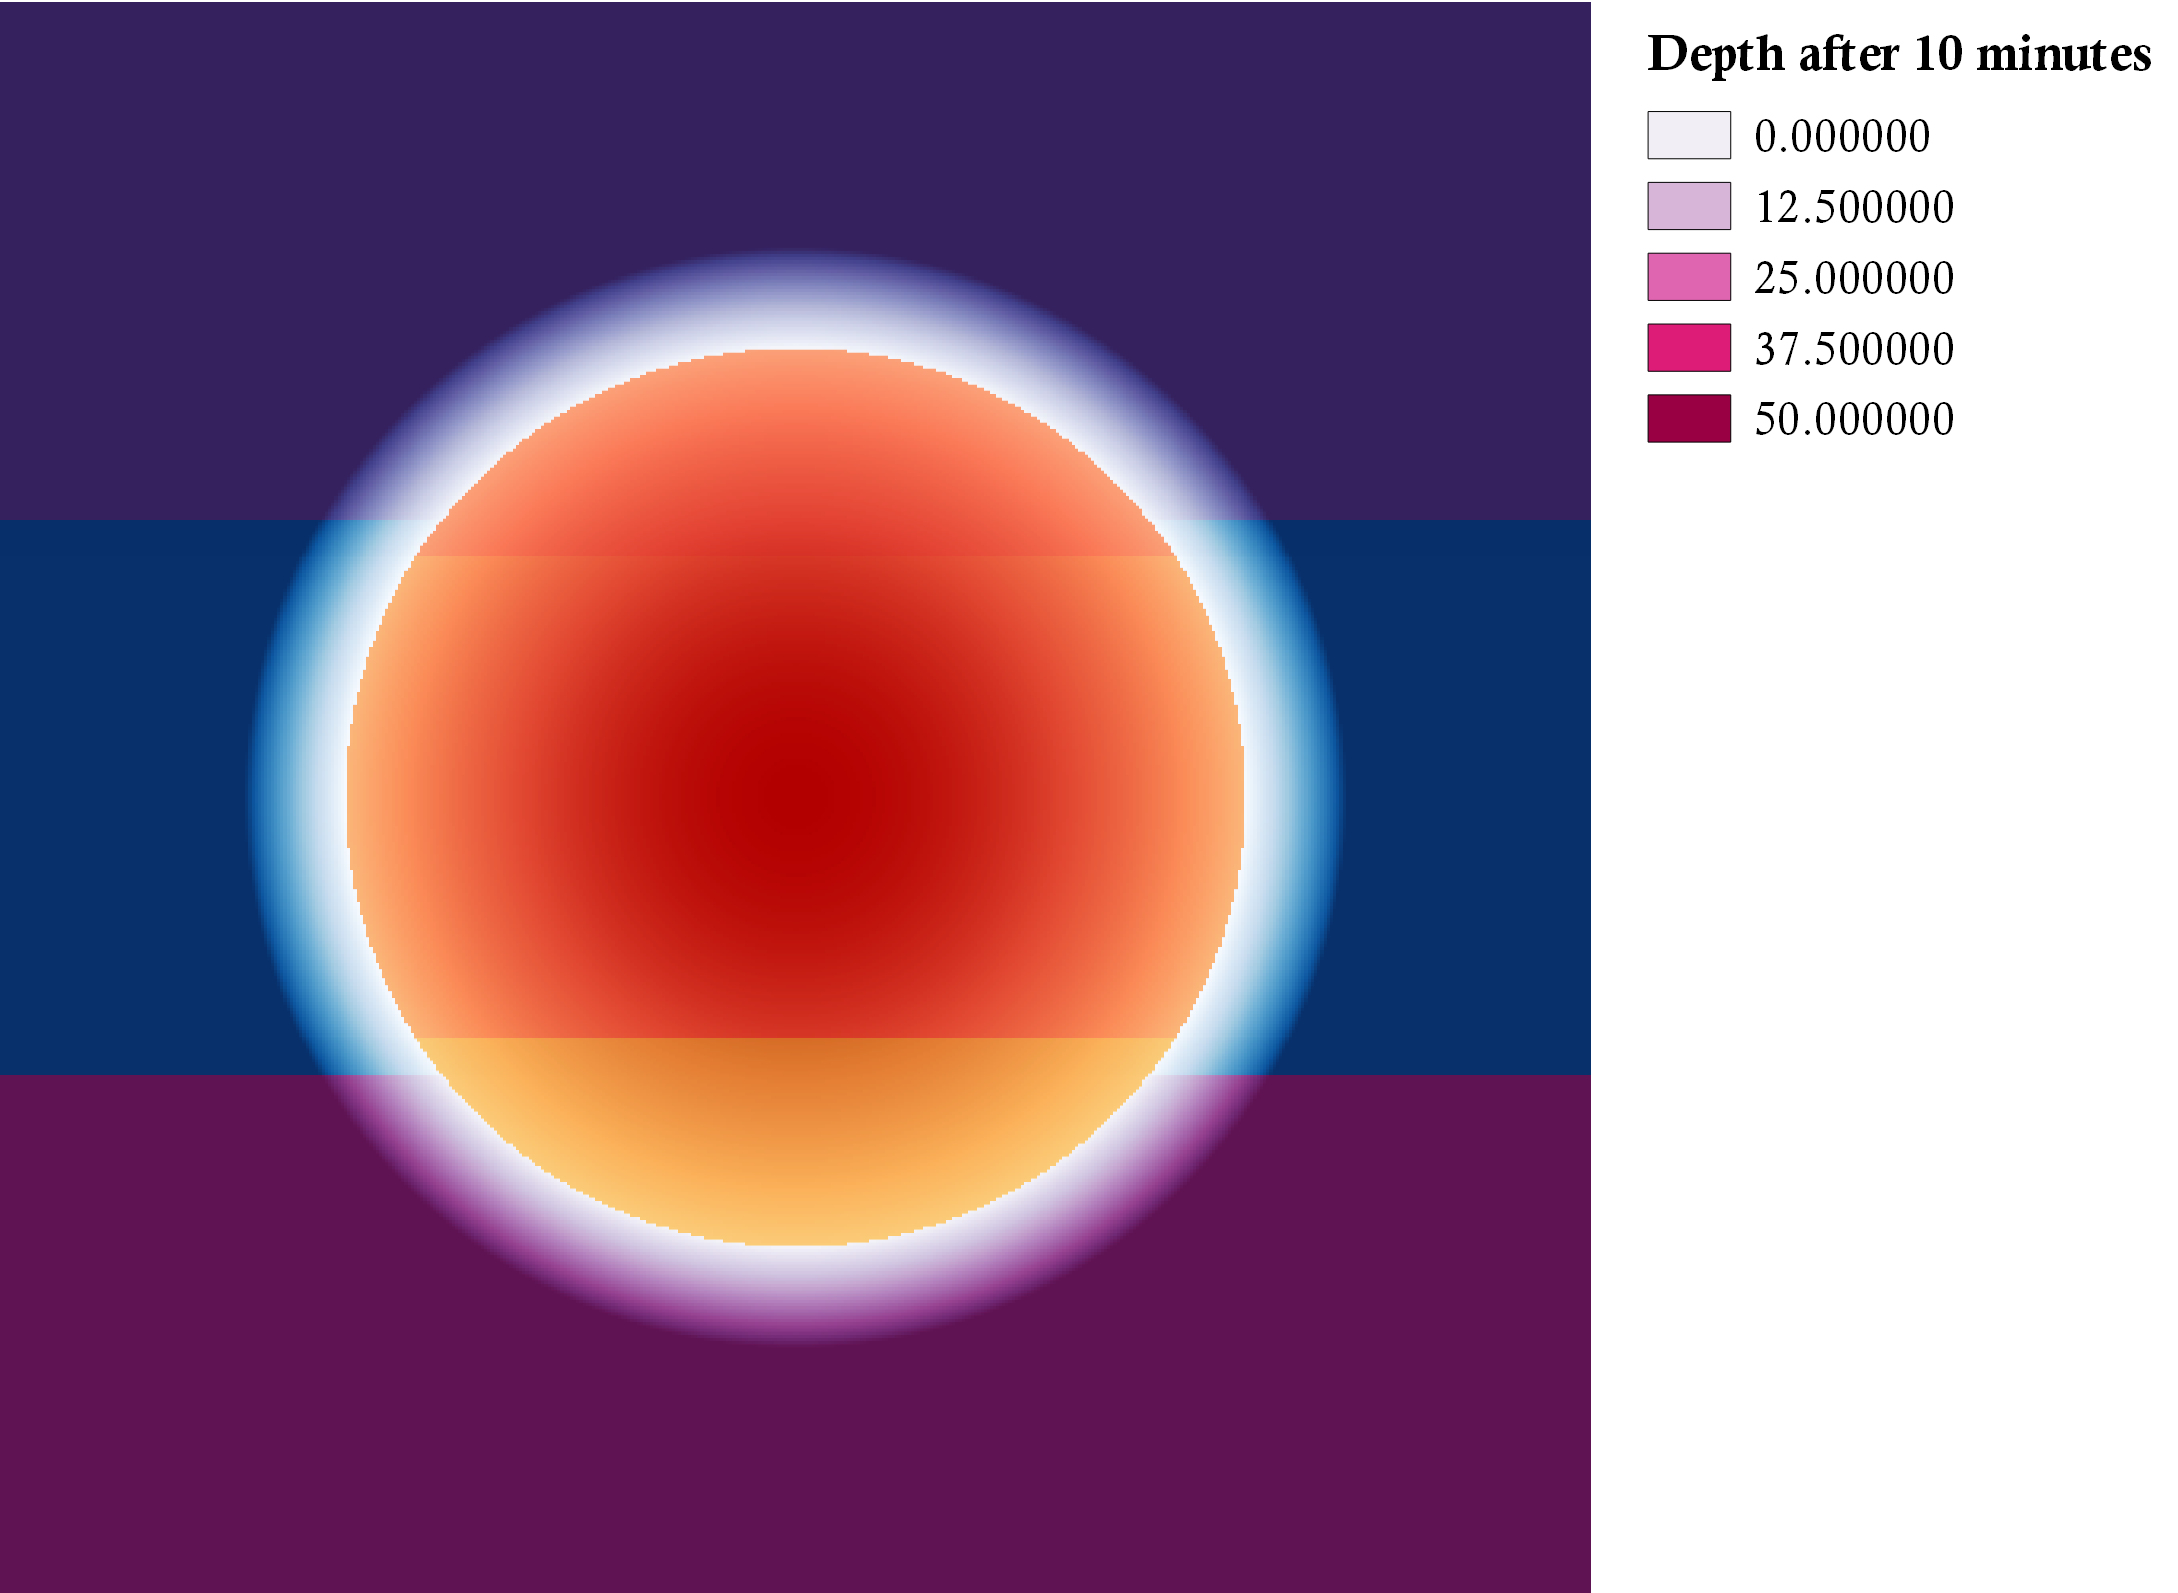
\includegraphics[width=0.85\textwidth]{decomposition-test-figures/static-lake-depth.png}
	\caption{Bed topography and depth after 10 minutes resulting from the static lake test with three devices, in which a tint has been applied to each of the subdomains to show the zones of overlap.}
	\label{TestResult_WellBalanced_Decomposed_Depth}
\end{figure*}
\begin{table*}[p]
	\small
	\centering
	\caption{Simulation run-times with different numbers of NVIDIA Tesla K40 devices, for the well-balanced property test, using the first-order Godunov-type and second-order MUSCL-Hancock schemes (hh:mm:ss)}
	\label{PerformanceResults_MultiGPU_WellBalanced}
	\begin{tabular}{p{0.15\linewidth}p{0.3\linewidth}p{0.1\linewidth}p{0.15\linewidth}p{0.15\linewidth}}
		\hline
		\multicolumn{5}{c}{\textbf{Performance results for well-balanced test (hh:mm:ss)}} \\
		\hline
		Resolution		 	& Productive cells					& Devices	& First-order	& Second-order	\\
		\hline
		8.0m				& 15,625 ($125 \times 125$)			& 1			& 00:00:01		& 00:00:01	\\
		&									& 2			& 00:00:01		& 00:00:01	\\
		&									& 3			& 00:00:01		& 00:00:01 	\\
		\hline
		4.0m				& 62,500 ($250 \times 250$)			& 1			& 00:00:02		& 00:00:02	\\
		&									& 2			& 00:00:02		& 00:00:02	\\
		&									& 3			& 00:00:02		& 00:00:02	\\
		\hline
		2.0m				& 250,000 ($500 \times 500$)		& 1			& 00:00:07		& 00:00:09 	\\
		&									& 2			& 00:00:05		& 00:00:06	\\
		&									& 3			& 00:00:06		& 00:00:07  \\
		\hline
		1.0m				& 1,000,000 ($1000 \times 1000$)	& 1			& 00:00:43		& 00:01:01	\\
		&									& 2			& 00:00:27		& 00:00:36	\\
		&									& 3			& 00:00:22		& 00:00:29	\\
		\hline
		0.5m				& 4,000,000 ($2000 \times 2000$)	& 1			& 00:05:14		& 00:07:45	\\
		&									& 2			& 00:02:46		& 00:04:02	\\
		&									& 3			& 00:02:10		& 00:03:02	\\
		\hline
		0.25m				& 16,000,000 ($4000 \times 4000$)	& 1			& 00:41:02		& 01:01:21	\\
		&									& 2			& 00:20:55		& 00:31:12	\\
		&									& 3			& 00:16:02		& 00:23:08	\\
		\hline
	\end{tabular}
\end{table*}

When the domain is divided in two, the island is also divided, hence the processing load for each device should be identical. Division of the domain into three creates a central domain, in which the island resides, where fewer cells require flux calculation; accordingly, one device has a reduced workload, but the software should be capable of addressing this, and where timesteps are synchronised between domains, the slowest domain becomes the governing factor. Figure \ref{TestResult_WellBalanced_Decomposed_Domains} shows the domain divided into three.

No movement in the water level is expected, for any duration of time. This behaviour is confirmed in the results shown in Figure \ref{TestResult_WellBalanced_Decomposed_Depth}, which confirms the synchronisation procedures in the software are correctly mapping the overlapping cells during data transfer.

The domain is $1000 \times 1000m$, and ten rows of cells form the overlap between each fragment of the domain, meaning at least an additional five rows per device for each division introduced. Grid resolutions from $8.0m$ to $0.25m$ are evaluated, and timesteps are synchronised between domains for this test. Accordingly, each new device introduced increases the total number of cells requiring computation.

The total run-times are given in Table \ref{PerformanceResults_MultiGPU_WellBalanced}. With regard to strong scaling, for higher resolutions, a marked decrease in run-time is shown for an increasing number of processing devices. The scaling is not linear, with the run-time at $0.25m$ resolution approximately $2.56\times$ lower for first-order, and $2.65\times$ for second-order. This is expected: the domain sizes are not sufficiently large to alleviate the overhead associated with synchronisation, most notably the requirement to transfer the timestep information across the host bus following each iteration of the scheme. The slightly larger factor of improvement for second-order corresponds to the increased workload within the scheme itself, and thus the smaller proportion of time consumed by simulation coordination. This is consistent with the findings of \citet{Saetra2012}, where the total domain size exceeded $40M$ cells before near-linear scaling was observed. Using multiple GPUs only seemingly becomes worthwhile in this case for $16M$ cells and beyond, with very little benefit at lower numbers of cells. This poses a problem for many simulations which are applied today, for which the problem is often the duration of the simulation rather than the number of grid cells, for which multiple processing devices can offer little benefit.

\subsection{Moving wet-dry fronts}

The sloshing parabolic bowl test, previously used in Chapter \ref{chapter:NumericalValidation} provides a different problem for the software to address. In this simulation, the velocities are constantly changing, and when the domain is divided, different CFL constraints are likely to exist in each component. Considering the requirement for extremely large numbers of cells to fully leverage the processing power available, this simulation uses grid resolutions ranging from $20m$ to $1.25m$ for a $10,000 \times 10,000m$ domain, hence up to $64M$ cells.

Results at different times during the test simulation using the MUSCL-Hancock scheme, with two domains, are shown in Figure \ref{TestResult_ParabolicBowl_2O_Decomposed2}. These clearly correspond to the expected results previously shown for a single domain in Figure \ref{TestResult_ParabolicBowl_2O}. Results using both explicit timestep synchronisation, and the decoupled forecasted method produce near-identical results, with some minor differences in water level but no change to the overall behaviour. These results demonstrate the software's capacity to correctly simulate the complex condition of constantly moving wet-dry fronts, even when these conditions occur along the divide between two subdomains. Simulations were also conducted using a first-order scheme, for performance comparisons only, as the results are known to deviate significantly from the analytical solution due to numerical diffusion. 

\begin{figure*}[tpb]
	\centering
	\begin{tabular}{cc}
		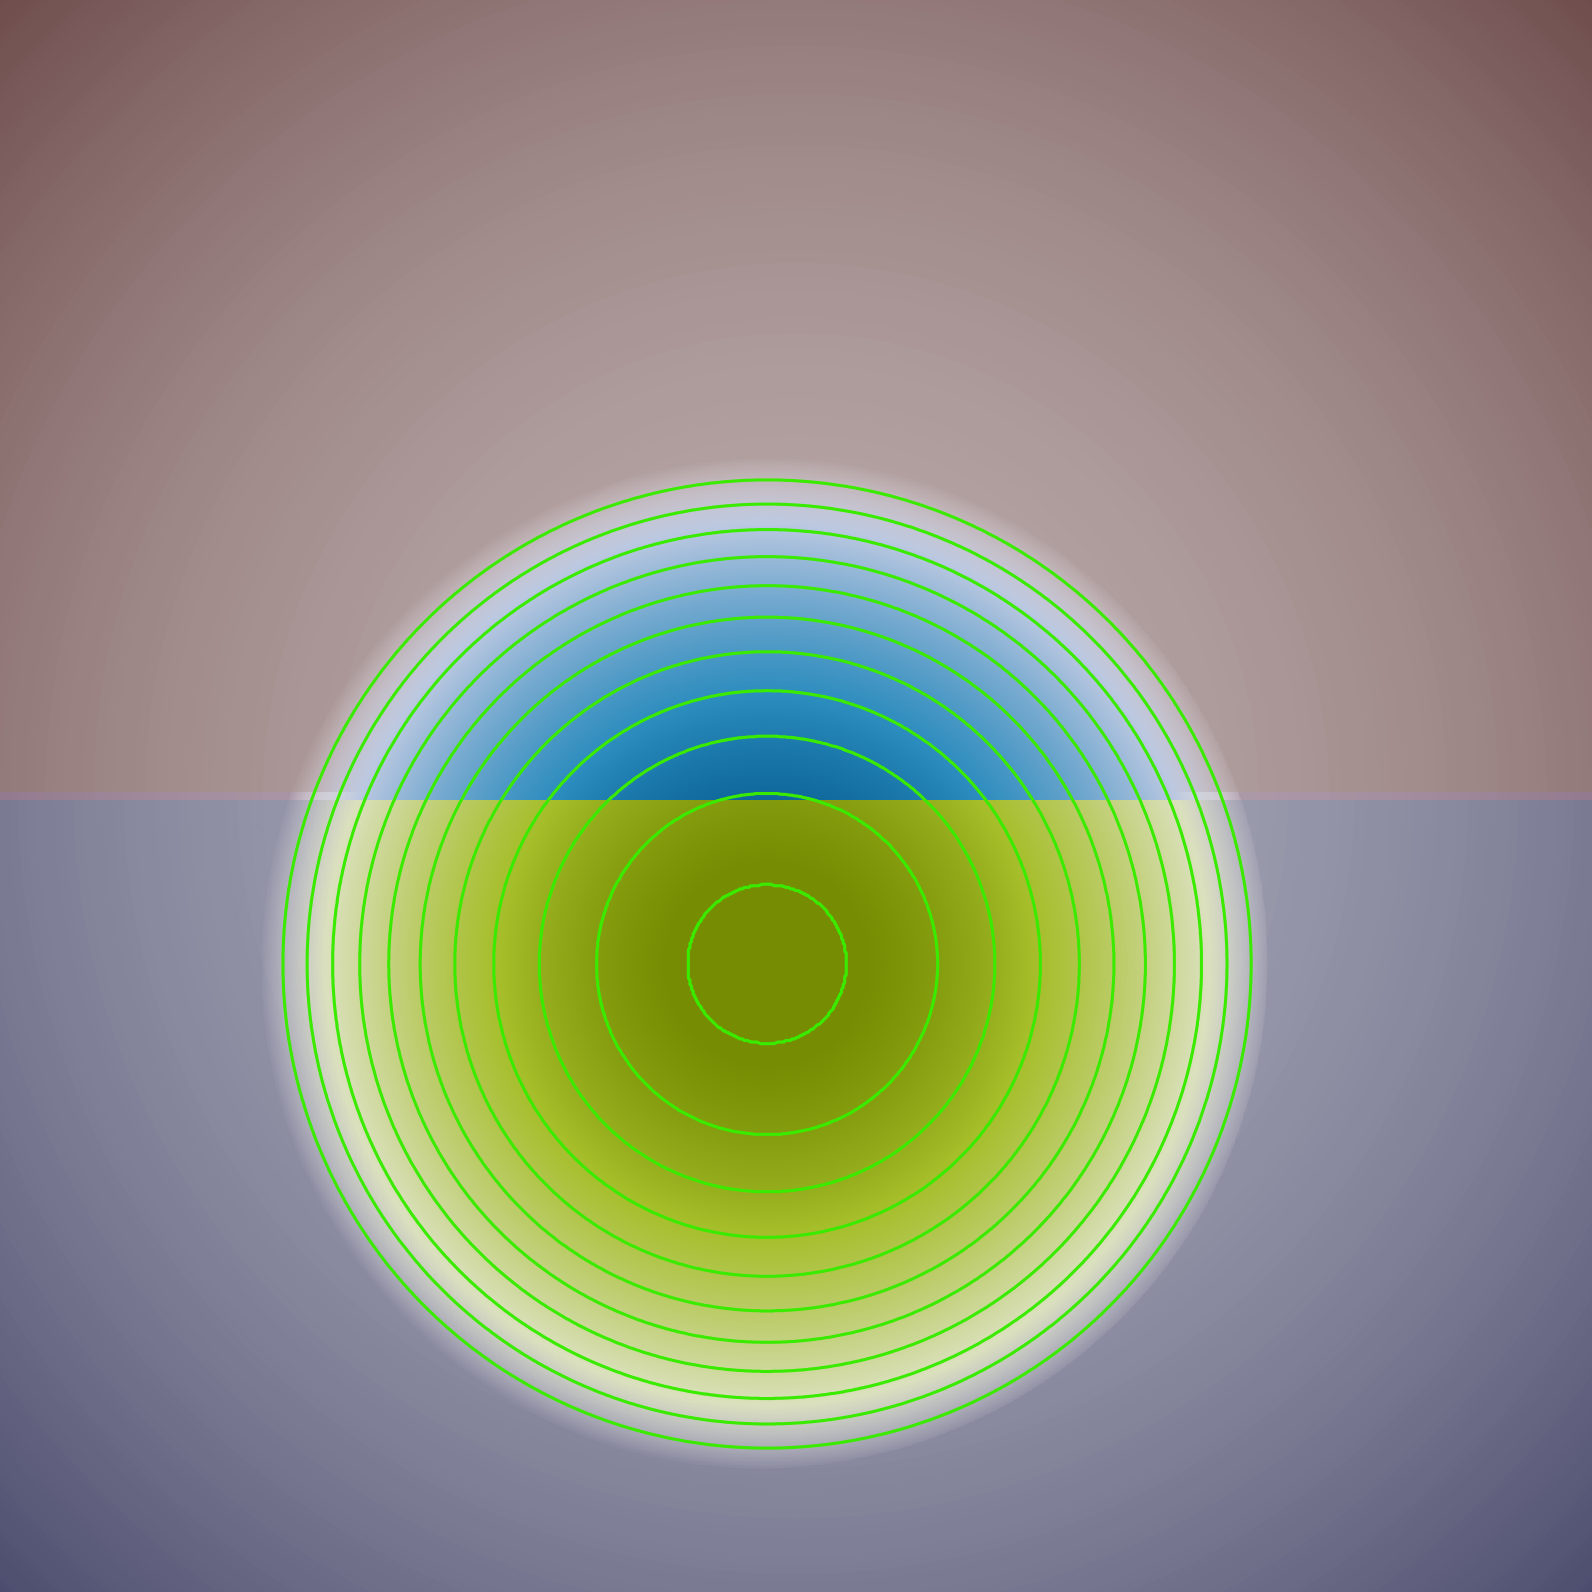
\includegraphics[width=0.4\textwidth]{decomposition-test-figures/parabolic-bowl-2O-2D-depth-300s.png} &
		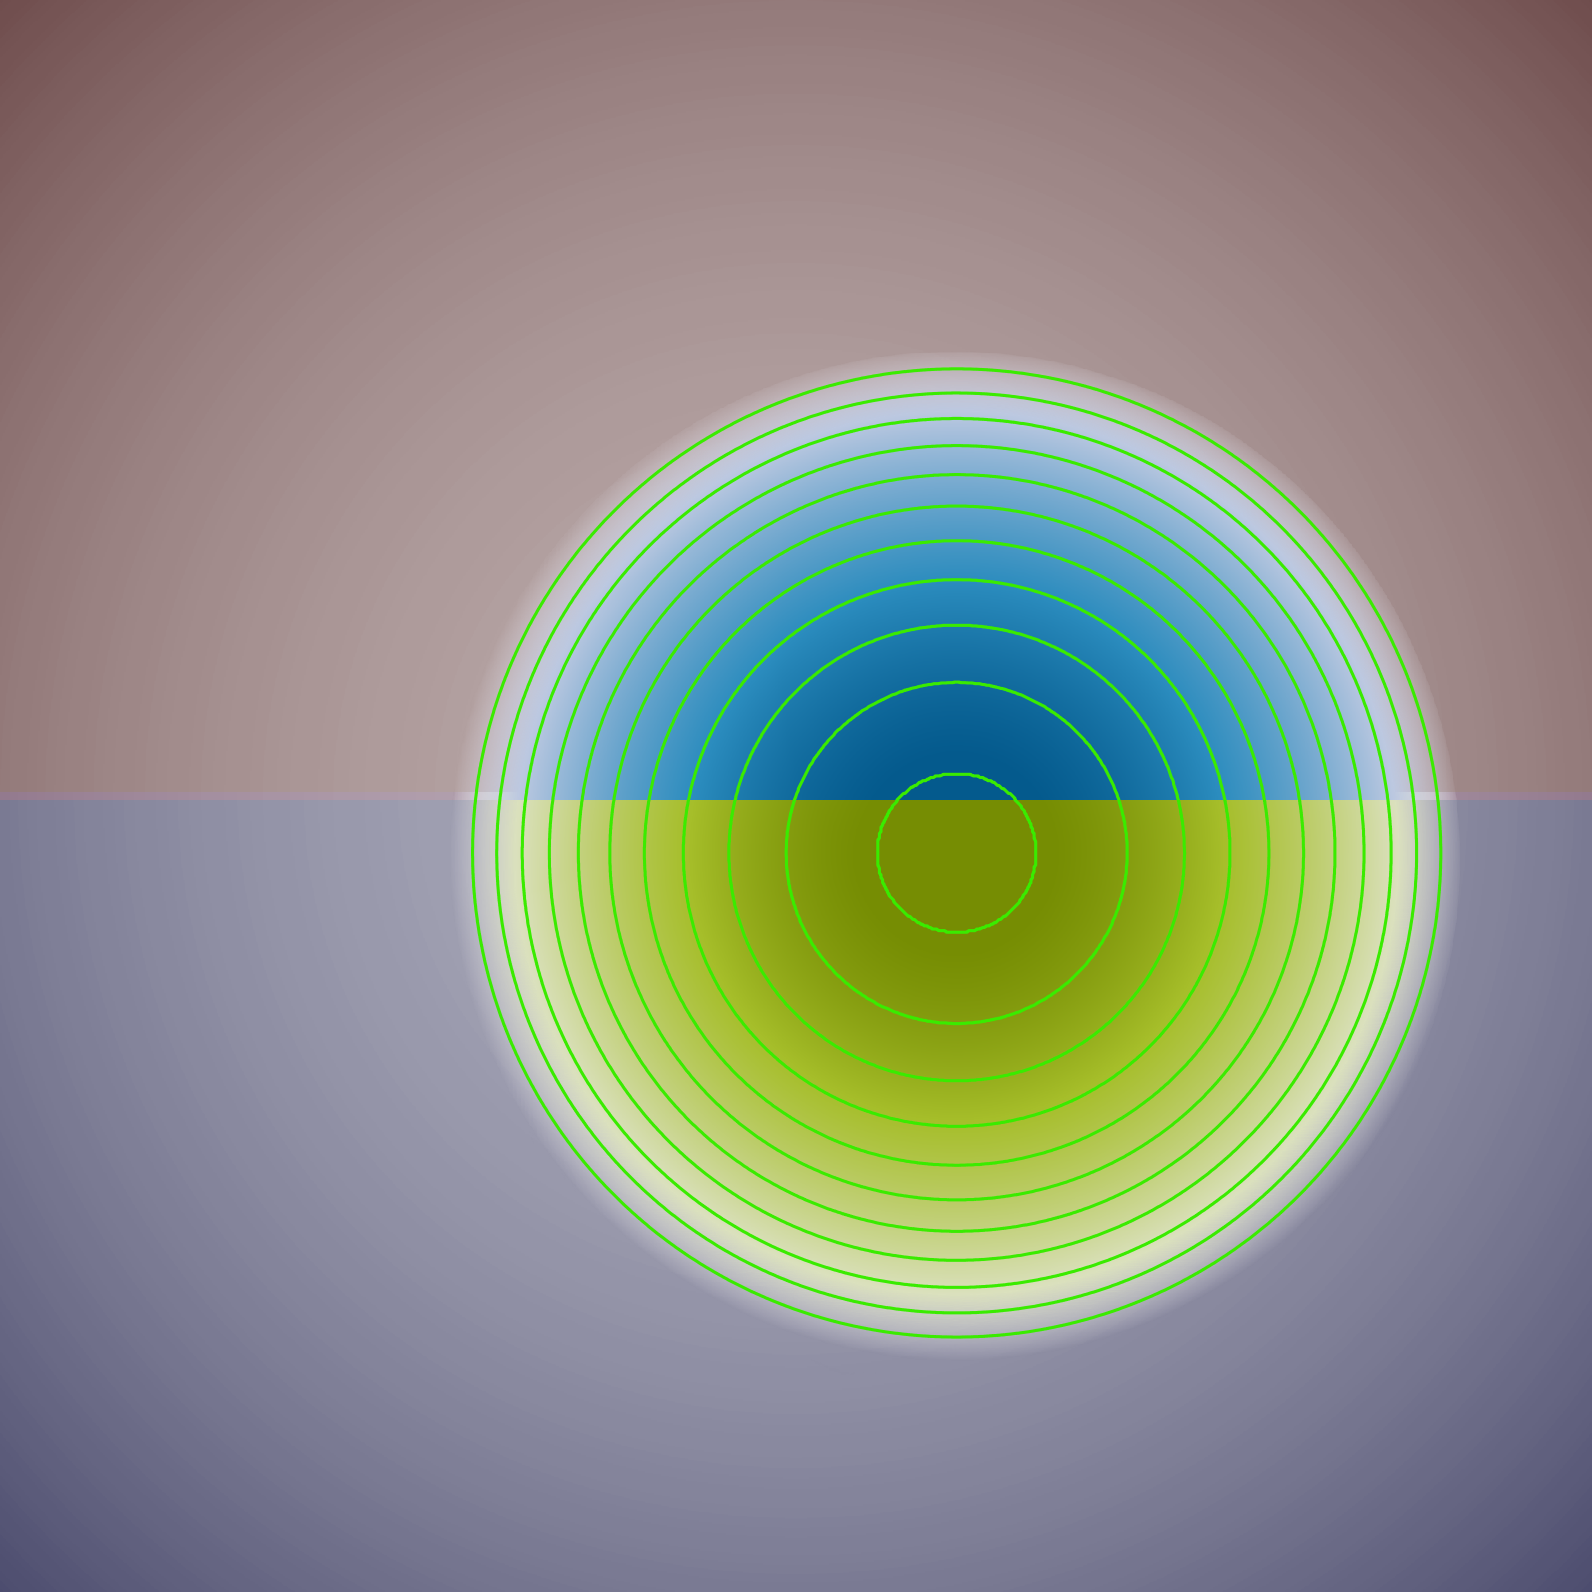
\includegraphics[width=0.4\textwidth]{decomposition-test-figures/parabolic-bowl-2O-2D-depth-600s.png} \\
		(a) 300s &
		(b) 600s \\[6pt]
		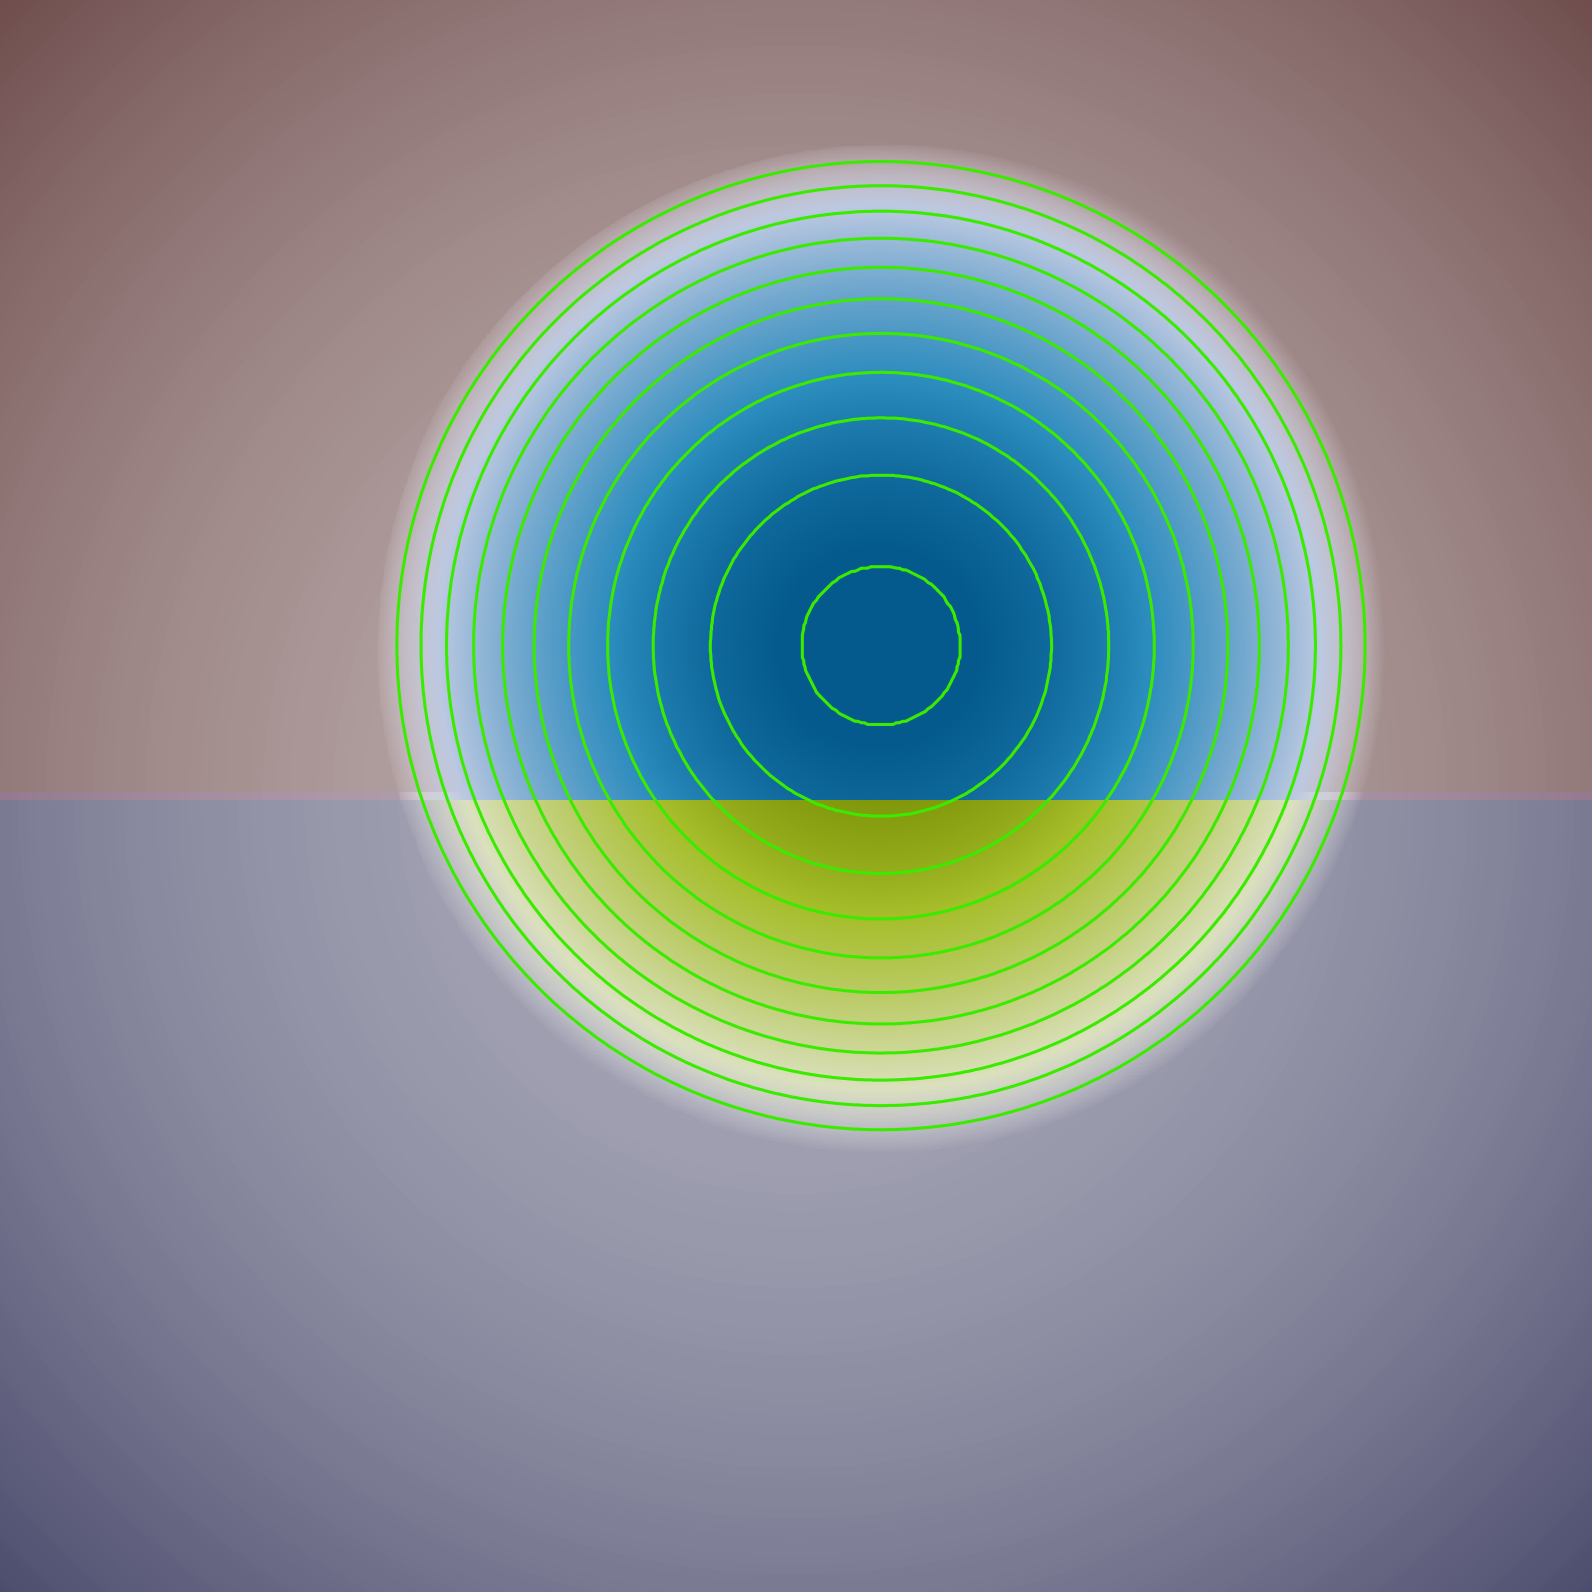
\includegraphics[width=0.4\textwidth]{decomposition-test-figures/parabolic-bowl-2O-2D-depth-900s.png} &
		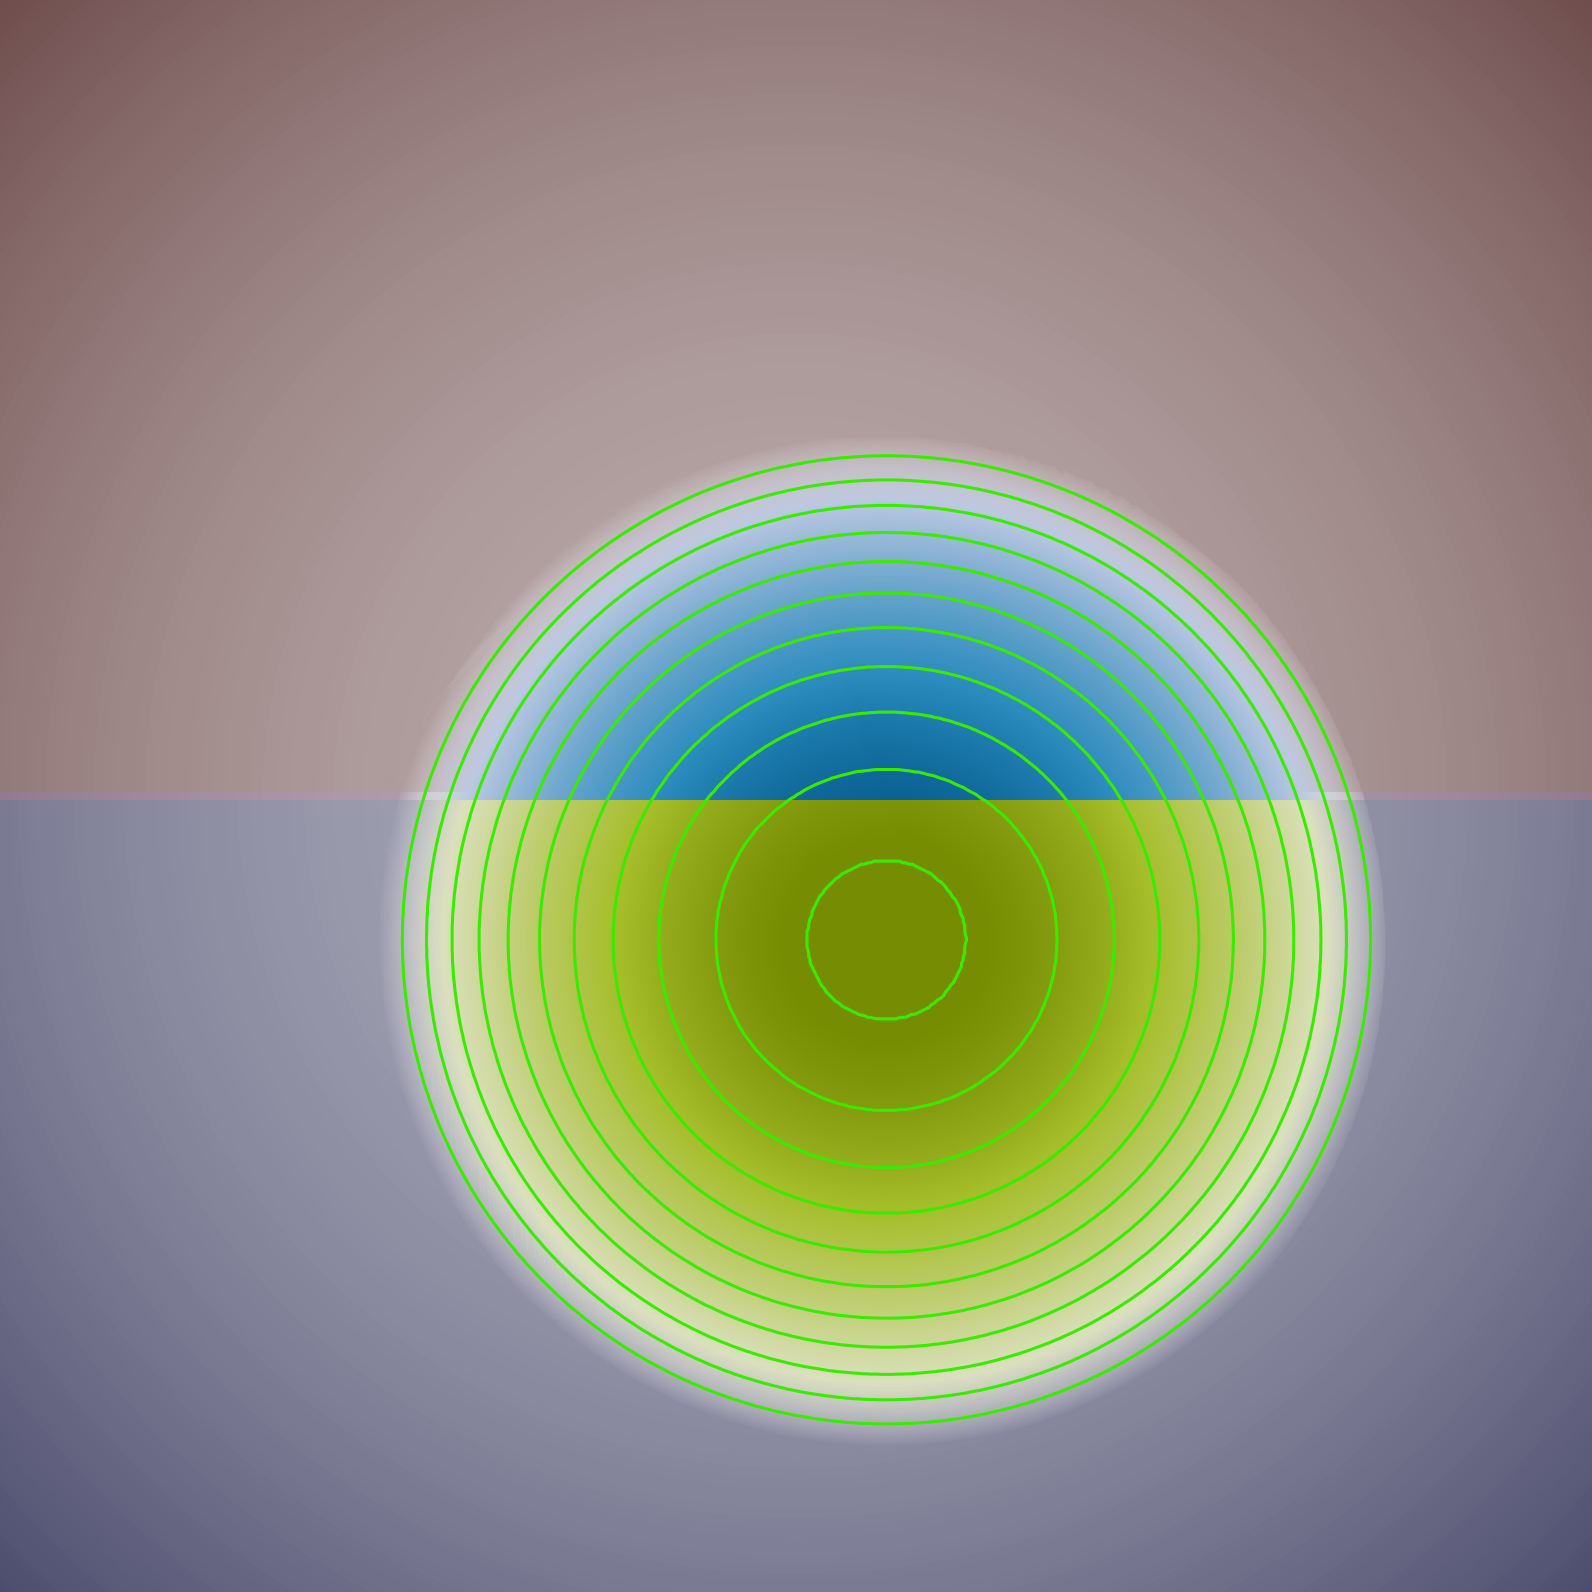
\includegraphics[width=0.4\textwidth]{decomposition-test-figures/parabolic-bowl-2O-2D-depth-1800s.png} \\
		(c) 900s &
		(d) 1800s \\[6pt]
		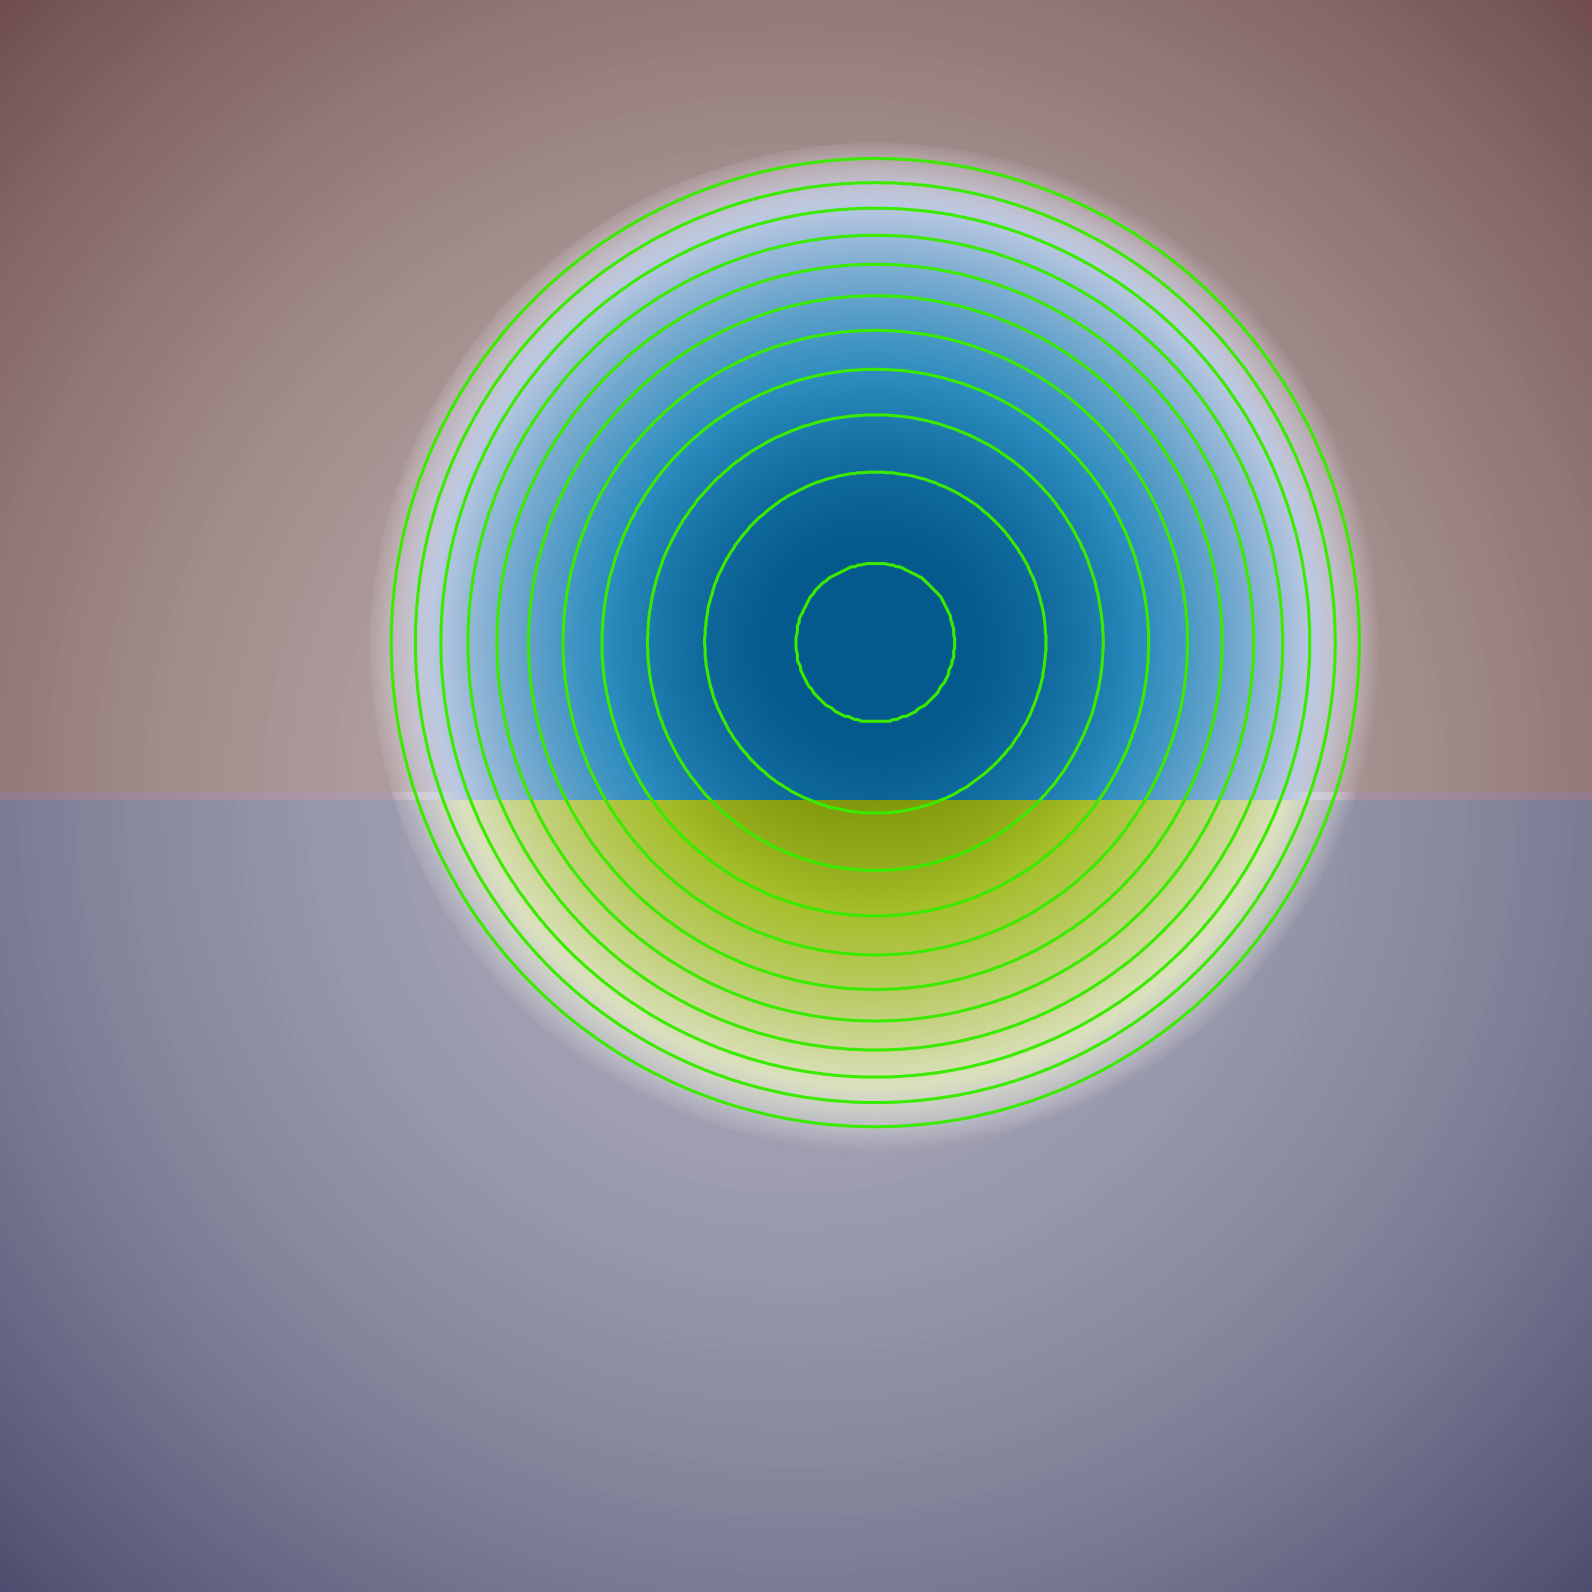
\includegraphics[width=0.4\textwidth]{decomposition-test-figures/parabolic-bowl-2O-2D-depth-3600s.png} &
		\\
		(e) 3600s &
	\end{tabular}
	\caption{Representative times for the parabolic bowl results for comparison against Figure \ref{TestResult_ParabolicBowl_2O}, with the domain decomposed down the middle, and the depths and bed topography tinted to reflect the processing device responsible.}
	\label{TestResult_ParabolicBowl_2O_Decomposed2}
\end{figure*}
\begin{table*}[p]
	\small
	\centering
	\caption{Simulation run-times with different numbers of NVIDIA Tesla K40 devices, for the sloshing parabolic bowl test, using the first-order Godunov-type and second-order MUSCL-Hancock schemes (hh:mm:ss) with 64-bit floating point}
	\label{PerformanceResults_MultiGPU_SloshingBowl}
	\begin{tabular}{p{0.15\linewidth}p{0.3\linewidth}p{0.1\linewidth}p{0.15\linewidth}p{0.15\linewidth}}
		\hline
		\multicolumn{5}{c}{\textbf{Performance results for sloshing parabolic bowl (hh:mm:ss)}} \\
		\hline
		Resolution		 	& Productive cells						& Devices	& First-order	& Second-order	\\
		\hline
		20.0m				& 250,000 ($500 \times 500$)			& 1			& 00:00:01		& 00:00:18	\\
		&															& 2			& 00:00:01		& 00:00:15	\\
		&															& 3			& 00:00:01		& 00:00:13 	\\
		\hline
		10.0m				& 1,000,000 ($1000 \times 1000$)		& 1			& 00:01:05		& 00:01:54	\\
		&															& 2			& 00:00:42		& 00:01:09	\\
		&															& 3			& 00:00:39		& 00:00:57	\\
		\hline
		5.0m				& 4,000,000 ($2000 \times 2000$)		& 1			& 00:07:44		& 00:13:39 	\\
		&															& 2			& 00:04:14		& 00:07:18	\\
		&															& 3			& 00:03:43		& 00:05:45  \\
		\hline
		2.5m				& 16,000,000 ($4000 \times 4000$)		& 1			& 00:59:58		& 01:47:07	\\
		&															& 2			& 00:31:27		& 00:55:58	\\
		&															& 3			& 00:27:06		& 00:43:45	\\
		\hline
		1.25m				& 64,000,000 ($8000 \times 8000$)		& 1			& 07:56:11		& \textit{N/A}	\\
		&															& 2			& 04:05:55		& 07:14:53	\\
		&															& 3			& 03:27:58		& 05:36:40	\\
		\hline
	\end{tabular}
\end{table*}

It was not possible to simulate the $1.25m$ grid using the MUSCL-Hancock scheme on a single device, as the NVIDIA Tesla K40 has insufficient memory to hold the intermediate data. The ability to run simulations exceeding the capacity of a single device is nonetheless an additional benefit of the domain decomposition approach. There is evidence that at the tens of million cell scale, strong scaling is approaching linearity. The first-order run-time is reduced by $48.4\%$ using two devices instead of one. The scaling is less ideal for three devices, but an even larger domain would likely achieve scaling improvements. Consistent with the previous results in this chapter, decomposition is shown to only be worthwhile for extremely large domains.

\section{Performance of forecasted and coupled implementations}

The results presented thus far focus on simulations in which the timesteps are synchronised between all domains, which is the simplest and most reliable method of domain decomposition available in the software. It is also possible to temporally-decouple the simulations, so their timesteps are independent and data is synchronised at a forecasted point in the future. The aforementioned tests in this chapter all produced comparable (although not identical) results using both methods of synchronisation; the differences are derived from the different timesteps and number of iterations, and consequent minor difference in the numerical diffusion. 

\begin{table*}[p]
	\small
	\centering
	\caption{Simulation run-times with forecasted and coupled runs of first 10 minutes of the sloshing bowl test using the second-order scheme (hh:mm:ss)}
	\label{PerformanceResults_MultiGPU_ForecastMethods}
	\begin{tabular}{p{0.15\linewidth}p{0.1\linewidth}p{0.35\linewidth}p{0.15\linewidth}}
		\hline
		\multicolumn{4}{c}{\textbf{Performance comparison for methods of synchronisation (hh:mm:ss)}} \\
		\hline
		Resolution		 	& Devices	& Synchronisation				& Run-time \\
		\hline
		5.0m				& 2			& Coupled timesteps				& 00:01:14 	\\
							& 2			& Forecasted synchronisation	& 00:01:37	\\
		\hline
		2.5m				& 2			& Coupled timesteps				& 00:08:58	\\
							& 2			& Forecasted synchronisation	& 00:11:14	\\
		\hline
		1.25m				& 2			& Coupled timesteps				& 01:10:00	\\
							& 2			& Forecasted synchronisation	& 01:27:43	\\
		\hline
	\end{tabular}
\end{table*}

Simulation run-times for the first 600 seconds of the sloshing parabolic bowl simulation are given in Table \ref{PerformanceResults_MultiGPU_ForecastMethods}, in which the forecasted method is markedly slower than timestep synchronisation. There are a number of reasons for this: the forecasted synchronisation point means sometimes kernels are scheduled which cannot perform flux computation, but the overhead associated with running the kernel remains present; some of the simulation may be repeated because of a rollback, if the forecast was inaccurate; and the additional time taken to download an entire copy of the cell state data after each successful batch of scheme iterations. 

For simulations in which the workload is comparable in all domains (e.g. the tests used herein, or a pluvial rainfall event in which all cells are engaged in computation), then timestep synchronisation is recommended. The forecasted method potentially may provide performance benefits in select cases, such as balancing hardware resources which do not have equal computational power, or when the domain is decomposed such that one domain contains a far greater proportion of wet cells, or far higher depths, than the remaining domains.

\section{Conclusions}

This chapter presented the background and algorithms associated with domain decomposition in the new software, where a single domain may be split into a number of horizontal components, with each addressed by a different processing device. This allowed simulations exceeding the memory available on a single device, and reduced the run-time of simulations, in some cases achieving near-linear run-time reduction for the number of devices added.

\begin{itemize}
	\item Many of the simulations used in practical engineering applications at present, are too small to fully benefit from domain decomposition to multiple heterogeneous devices. In particular, long duration simulations as opposed to large spatial extents, cannot be accelerated using the decomposition methods herein.
	\item Decomposed elements of a domain may share a single timestep or be independent, by predicting a point in the future to synchronise data, however there are but a handful of circumstances in which the latter would be a more expedient option, as the additional complexity involved carries a performance cost.
	\item Results obtained through the decomposition methods are near-identical (to at least three significant figures) to those from a single processing device, and do not inhibit the capabilities of the numerical scheme discussed in Chapter \ref{chapter:NumericalMethods}.
	\item Simulations which require processing power exceeding that which may be provided by a single server, can use the new software to leverage multiple servers, using MPI for internodal communication.
\end{itemize}

This chapter only considered the methods, and validity of results obtained therewith, for domain decomposition. The approach must therefore be applied to a real-world case, which would not be feasible to simulate without the assistance of multiple heterogeneous processing devices.